\documentclass[11pt,a4paper]{article}

\usepackage[margin=2.4cm]{geometry}
\usepackage{graphicx}
\usepackage{booktabs}
\usepackage{amsmath,amssymb}
\usepackage{xcolor}
\usepackage{listings}
\usepackage[colorlinks=true,linkcolor=black,urlcolor=blue,citecolor=black]{hyperref}
\usepackage{caption}
\usepackage{array}
\usepackage{longtable}

\graphicspath{{figures/}}
\captionsetup{font=small,labelfont=bf}
\setlength{\parskip}{0.4em}
\setlength{\parindent}{0pt}
\setlength{\emergencystretch}{3em}  % avoid overfull lines from long \texttt identifiers

\definecolor{good}{RGB}{42,157,143}
\definecolor{bad}{RGB}{209,73,91}
\definecolor{warn}{RGB}{233,155,60}
\newcommand{\ok}{\textcolor{good}{\textbf{OK}}}
\newcommand{\susp}{\textcolor{bad}{\textbf{SUSPECT}}}
\newcommand{\und}{\textcolor{warn}{\textbf{undecidable}}}

\lstset{basicstyle=\ttfamily\footnotesize,frame=single,breaklines=true,
        backgroundcolor=\color{black!3},columns=fullflexible}

\title{\textbf{Video Data Quality in Centri}\\[0.3em]
\large A Per-Phenomenon Breakdown of Tracking and Projective Artifacts\\
in Automatically Generated Circular-Motion Learning Material}
\author{Technical Report --- Centri / Hwang Lab}
\date{2026-07-15\quad(rev.\ 2026-07-16: fan blade-tip scale measured, SILVER tier, $\omega(t)$ staircase fix)}

\begin{document}
\maketitle

\begin{abstract}
\noindent
Centri generates physics learning material from smartphone video of circular motion. Its
kinematic curves are visibly ragged where the parent system's (P-MAGIC) are a clean line.
This report establishes the cause per phenomenon across the full 11-template corpus.

Two findings dominate. First, on one clip (\texttt{roundabout-4046}) \textbf{the ragged
$\omega(t)$ is not noise and not tilt: it is true perspective projection}. The natural remedy
(fit the elliptical image of the orbit, stretch it back to a circle) removes only $12\%$ of it,
because an affine model addresses the wrong harmonic. An uncalibrated projective rectification,
derived from the imaged rotation axle and the orbit conic, removes $91\%$ (ripple CV
$0.166 \rightarrow 0.015$) while leaving mean $\omega$ invariant to four significant figures.

Crucially, \textbf{this does not generalise, and the reason is the useful result}. Applying the
same rectification to the two other clips that a tilt-based reading nominates
(\texttt{bicycle}, \texttt{turntable-1}) changes nothing, correctly. \textbf{Perspective
strength is the offset between the imaged axle and the centre of the elliptical path --- not
the tilt.} That offset is $85.6$\,px on 4046 and $0.7$--$8.8$\,px on every other clip, an order
of magnitude apart. All of these clips are tilted $15$--$27^\circ$; tilt determines only that
the orbit \emph{images} as an ellipse, not that the projection is perspective rather than
affine. An earlier draft of this report claimed the artifact was corpus-wide; that claim was
produced by a classifier that read the harmonic ratio without checking whether the ripple was
phase-locked at all, and it is retracted in \S\ref{sec:null}.

Second, \textbf{detection fails on $\sim$20\% of the corpus, always by the same mechanism}: the
text prompt matches a background object of the same shape or colour. \texttt{"fan blade"}
tracks window louvres; \texttt{"black knob"} tracks foliage. These clips report
\texttt{track\_coverage: 1.0} while being wrong in over a third of frames.

Third, \textbf{the two clips whose curves looked cleanest were not measurements at all}: their
orbits are synthesized by \texttt{frequency} mode, which carries a floor at $1.0$\,rad/s and so
reports the fan spinning while it is provably at rest ($0.002$\,rad/s). The blade-pass \emph{rate}
is nonetheless correct (verified against the real red marker, correlation $0.974$); measuring the
blade-tip scale with a ruler ($559$\,px/m) and interpolating the FFT bins to remove a quantisation
staircase make $v$, $a_c$ and $\omega(t)$ trustworthy. But because the per-frame orbit is
reconstructed from the rate, these clips are \textbf{silver} --- teachable numbers, reconstructed
trajectory --- not gold.

Of four phenomena we can now vouch for, \textbf{only one required correcting the data}; the other
three were recovered by fixing our own diagnostics and configuration. We report what did
\emph{not} work --- including four of our own claims falsified by frame-by-frame inspection, and a
tracker bug we documented and then re-committed --- and locate each fix in the architecture:
geometry is deterministic and belongs in code, while per-clip judgement belongs to the agent.
\end{abstract}

\tableofcontents
\newpage

%======================================================================
\section{Motivation and scope}

The parent system produces $\omega(t)$ curves that read as a single clean line. Centri's, from
comparable phenomena, oscillate. Because the material generator narrates these curves to
students, the distinction is pedagogical, not cosmetic: on \texttt{roundabout-4046} the
uncorrected curve swings between $5.5$ and $12$\,rad/s roughly $18$ times in $15$ seconds,
which tells a student the wheel repeatedly speeds up and slows down. It does not; it coasts
smoothly from $9.4$ to $6.5$\,rad/s.

This report answers, per phenomenon: \emph{what is actually wrong, what fixes it, and what
cannot be fixed downstream at all.}

\subsection{A note on method: statistics did not survive contact with the frames}
\label{sec:method-note}

Two claims in the first draft of this investigation were quantitative, plausible, and wrong.
Both were produced by computing a statistic over a track nobody had looked at:

\begin{enumerate}
  \item \emph{``\texttt{roundabout-4048} is filmed at a $29^\circ$ tilt.''} This was a conic
  fitted to a point cloud consisting substantially of trees and shadows. The number described
  the tracker's failures, not the scene.
  \item \emph{``The orbit is an ellipse, so squash it back.''} Correct about the ellipse,
  wrong about the remedy (\S\ref{sec:affine}).
\end{enumerate}

Consequently this report enforces an order that the rest of the pipeline should adopt:
\textbf{detection is verified first, by overlaying the cached track on real frames; geometry is
computed only afterwards, and only for clips that pass.} A geometry number from an unverified
track is not a measurement. The same discipline caught two further errors in our own survey
tool (\S\ref{sec:survey-bugs}).

%======================================================================
\section{Diagnostic method}

\subsection{Detection gate}

For each clip, from the cached trajectory: coverage, the per-frame step distribution, and the
coefficient of variation of the detected bounding-box area. A rigid object's apparent size is
near-constant, so a wildly varying box area means the detector is switching targets.

\textbf{The step bound must be angular, not a fixed pixel count.} Our first gate flagged any
step over 100\,px as a teleport. That is wrong, and it produced a false accusation against
\texttt{computerfan-4029} (\S\ref{sec:4029}): at $r = 312$\,px and 4\,rev/s a \emph{correctly}
tracked marker moves 131\,px per frame. The meaningful quantity is the angle swept per frame:
below ${\sim}90^\circ$ the point is unambiguous, above $180^\circ$ the spin is aliased and
unrecoverable at that frame rate. 4029 peaks at $55^\circ$/frame. A pixel threshold cannot
distinguish a fast object from a teleporting one; only comparison against the physical
expectation ($\omega r/\mathrm{fps}$) can.

\subsection{The harmonic fingerprint}
\label{sec:fingerprint}

If $\omega(t)$ ripples, the cause is identified before anything is applied. We detrend $\omega$
against time (cubic), then regress the residual on harmonics of \emph{orbital phase}. The ratio
of the 1-per-revolution amplitude $A_1$ to the 2-per-revolution amplitude $A_2$ names the cause.
Each candidate has a distinct signature, established by simulating a known-uniform spin under
each distortion (Figure~\ref{fig:fingerprint}, left):

\begin{center}
\begin{tabular}{lll}
\toprule
$A_1/A_2$ & Cause & Remedy \\
\midrule
$\approx 0$ (pure 2/rev) & affine tilt (foreshortening only) & ellipse $\to$ circle axis stretch \\
$\approx 1$--$3$ (mixed) & \textbf{true perspective} & projective rectification (\S\ref{sec:method-rect}) \\
$\gg 10$ (pure 1/rev) & wrong rotation centre & re-fit the centre \\
no phase-lock, broadband & detector/centroid noise & improve detection \\
\bottomrule
\end{tabular}
\end{center}

The decisive property: \textbf{a phase-locked ripple is deterministic}. It repeats identically
every revolution, so no low-pass filter removes it without also destroying the real $\omega(t)$
trend it sits on. This is the most expensive available mistake at this stage, and
\S\ref{sec:filter} shows the pipeline currently makes a version of it.

Two guards matter. The classification requires \textbf{at least 2 revolutions} of phase
coverage --- below that, $A_1$ and $A_2$ are not separable and the clip is reported
\und{} rather than clean. And all quantities are computed over the \textbf{active window}
only; a clip that idles then moves otherwise divides its ripple by a near-zero mean $\omega$
and reports a fictitious artifact.

\begin{figure}[htbp]
\centering
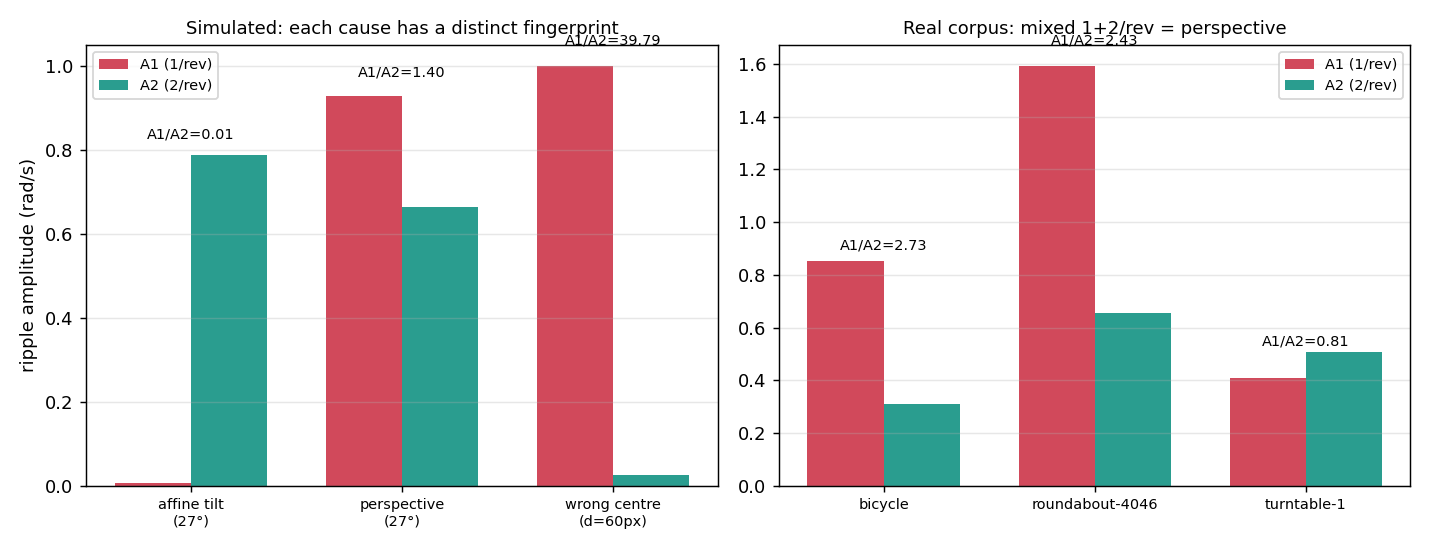
\includegraphics[width=\linewidth]{fig-fingerprint.png}
\caption{The harmonic fingerprint. \textbf{Left:} a simulated uniform spin under each candidate
distortion. Affine tilt produces almost pure 2/rev; a wrong centre produces almost pure 1/rev;
true perspective produces a mixture. \textbf{Right:} the real corpus. All three diagnosable
clips show the mixed signature of perspective. Amplitudes are read from the survey output, not
hand-entered.}
\label{fig:fingerprint}
\end{figure}

\subsection{How the numbers are computed}
\label{sec:howcomputed}

Every quantity reported per phenomenon is one of a small, fixed set. They are defined here once;
the per-clip sections then only state values. All are computed by the frozen \texttt{analysis/}
pipeline from a single input file (\texttt{pipeline\_inputs.json}); none is re-derived by the
agent (\S\ref{sec:filter}).

\paragraph{From pixels to metres.} The tracker returns a per-frame centroid $(x_t, y_t)$ in
pixels and a per-frame bounding box. One reference object of known real size sets the scale:
\begin{equation}
\mathrm{px\_per\_m} \;=\; \frac{d_{\mathrm{px}}}{s_{\mathrm{m}}},
\qquad
r_{\mathrm{m}} \;=\; \frac{r_{\mathrm{px}}}{\mathrm{px\_per\_m}},
\label{eq:calib}
\end{equation}
where $d_{\mathrm{px}}$ is the reference's median imaged diameter and $s_{\mathrm{m}}$ its real
size (the sidecar's \texttt{physical\_size}). \textbf{Only $v$ and $a_c$ depend
on this scale}; every angular quantity below is scale-free, which is why a wrong or missing
\texttt{physical\_size} leaves $\omega$, $T$ and $f$ untouched.

\paragraph{Angle, angular velocity, acceleration.} With the rotation centre $(c_x, c_y)$, the
orbital phase of the tracked point is
\begin{equation}
\theta_t \;=\; \operatorname{atan2}\!\left(y_t - c_y,\; x_t - c_x\right),
\end{equation}
unwrapped to a continuous $\theta(t)$. Angular velocity and acceleration are its first and second
time-derivatives, taken with a Savitzky--Golay filter (a sliding low-order polynomial fit) rather
than raw finite differences, so differentiation does not amplify pixel noise:
\begin{equation}
\omega(t) \;=\; \frac{d\theta}{dt}, \qquad \alpha(t) \;=\; \frac{d\omega}{dt}.
\end{equation}
Linear speed and centripetal (radial) acceleration of a point at radius $r$ follow from
rigid-body rotation:
\begin{equation}
v \;=\; \omega\, r, \qquad a_c \;=\; \omega^{2} r \;=\; \frac{v^{2}}{r}.
\label{eq:vac}
\end{equation}
Because $\omega$ is a property of the \emph{whole} rigid body --- identical at every radius --- once
$\omega$ is known, $v$ and $a_c$ may be evaluated at any chosen radius on the body. This is exact,
not an extrapolation: the fans report $v$ and $a_c$ at the blade tip using a ruler-measured tip
radius (\S\ref{sec:fans}). Figure~\ref{fig:onframe} shows every one of these quantities on a real
frame.

\begin{figure}[htbp]
\centering
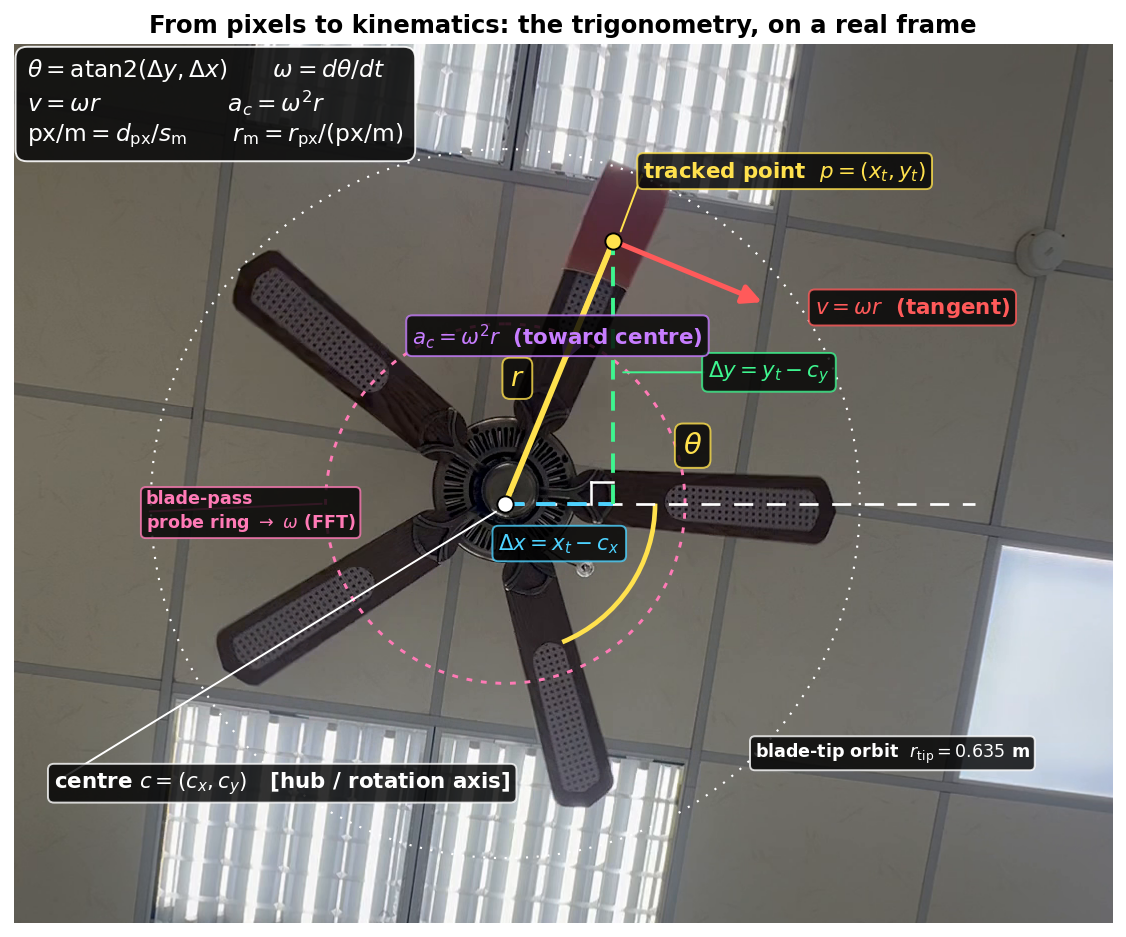
\includegraphics[width=\linewidth]{fig-formula-on-frame.png}
\caption{The equations of \S\ref{sec:howcomputed} on a real frame. The centre $c$ and a tracked
point $p$ define the legs $\Delta x, \Delta y$ of a right triangle, whose inverse tangent is the
orbital angle $\theta=\operatorname{atan2}(\Delta y,\Delta x)$; differentiating $\theta$ gives
$\omega$, and at radius $r$ the point has tangential speed $v=\omega r$ (red) and centripetal
acceleration $a_c=\omega^2 r$ toward the centre (purple). This trigonometric chain is what the
point-tracked clips (\texttt{roundabout-4046}, the turntables, \texttt{computerfan-4029}) use
directly. The frame here is a fan: for it $\omega$ instead comes from a windowed FFT of the
\textbf{blade-pass probe ring} (pink), but the \emph{same} radius geometry gives $v$ and $a_c$ at the
ruler-measured \textbf{blade-tip orbit} ($r_{\mathrm{tip}}=0.635$\,m, white).}
\label{fig:onframe}
\end{figure}

\paragraph{Period and frequency.} Over a stable-speed window,
\begin{equation}
T \;=\; \frac{2\pi}{\langle|\omega|\rangle}, \qquad f \;=\; \frac{1}{T},
\end{equation}
cross-checked against the dominant peak of the FFT of the phase (or of the probe signal below).

\paragraph{Frequency mode (bladed rotors).} Where no per-frame point survives --- identical,
motion-blurred blades --- $\omega$ is recovered \emph{without} tracking a point. Image intensity is
sampled at a ring of probes around the hub; each blade sweeping past a probe dips that signal. The
dominant frequency $f_b$ of the probe signal is the \emph{blade-pass} frequency, and with $N$
blades
\begin{equation}
f_{\mathrm{rot}} \;=\; \frac{f_b}{N}, \qquad \omega \;=\; 2\pi f_{\mathrm{rot}}.
\label{eq:bladepass}
\end{equation}
$f_b$ is read from a \emph{windowed} FFT (window $T_{\mathrm{win}}$, hop $h$), giving a
time-resolved $\omega(t)$ across spin-up and coast-down. An FFT resolves frequency only to
$\Delta f = 1/T_{\mathrm{win}}$, so taking the raw peak bin quantises $\omega$ into steps of
\begin{equation}
\Delta\omega \;=\; \frac{2\pi\,\Delta f}{N} \;=\; \frac{2\pi}{N\,T_{\mathrm{win}}},
\label{eq:quant}
\end{equation}
a non-physical staircase (for the fans, $N=5$, $T_{\mathrm{win}}=2.5$\,s $\Rightarrow
\Delta\omega \approx 0.5$\,rad/s). A three-point parabolic fit about the peak bin recovers the
sub-bin location and restores a smooth, physical $\omega(t)$ (\S\ref{sec:fans}).

\paragraph{Diagnostics.} An ellipse (conic) is least-squares fitted to the orbit; its semi-axes
$A \ge B$ give the \textbf{axis ratio} $A/B$ and an implied \textbf{tilt} $\arccos(B/A)$. The
\textbf{hub offset} is the distance between the imaged rotation axle and the centre of that ellipse
--- the quantity that actually measures perspective (\S\ref{sec:trap}), as distinct from tilt. The
\textbf{harmonic fingerprint} detrends $\omega$ and regresses the residual on harmonics of orbital
phase $\varphi$; the amplitudes $A_k$ of the $\cos(k\varphi)$ terms give the ratio $A_1/A_2$
(\S\ref{sec:fingerprint}). The \textbf{phase-lock fraction} is the share of ripple variance
explained by those phase harmonics ($1$ = perfectly orbit-locked, $0$ = broadband noise), and the
\textbf{ripple CV} is $\operatorname{std}(\omega)/\langle|\omega|\rangle$ over the active window.

\paragraph{What each clip hands the agent.} Two per-clip inputs steer the otherwise-generic
pipeline, and both are stated in each subsection below. The \textbf{sidecar} is a small JSON:
\texttt{tracking\_mode} (\texttt{object} = SAM3 text detection, \texttt{color} = HSV blob,
\texttt{frequency} = blade-pass), the detection \textbf{cue} noun(s), the \textbf{reference} object
and its \texttt{physical\_size}, the marked \texttt{rotation\_center\_frac}, and any
\texttt{tracking\_config} (HSV bounds, ROI, step limits). The injected \textbf{\texttt{hints.md}}
is prose substituted verbatim into the orchestrator prompt (\S\ref{sec:survey-bugs}). A wrong cue
noun or a missing \texttt{physical\_size} is the difference between a golden clip and a fabricated
one, so both are documented as the \emph{context handed to the agent}.

\subsection{Corpus}

Eleven templates, ten distinct videos, approximately six distinct phenomena. Two duplications
matter for any claim of generality:

\begin{itemize}
  \item \texttt{base-template-flick} and \texttt{basetemplate-turntable-3} are the
  \textbf{same clip}. Their cached tracks are byte-identical (350/350 points, both objects) and
  their sidecars share \texttt{rotation\_center\_frac} $[0.5028,0.4573]$. \texttt{flick} is
  \texttt{turntable-3}'s video re-skinned with a narrative \texttt{scene\_context}. The data
  genuinely shows a flick, so the re-skin is honest --- but the reference golden run
  (\texttt{9ed918d0}) is turntable-3's data.
  \item \texttt{turntable-1/2/3} are three clips of one phenomenon (a phone on a rotating base).
\end{itemize}

\textbf{Hazard.} \texttt{flick} ships a cached track but \emph{no video}. Because a cache hit
short-circuits tracking entirely, any video uploaded against that template silently reports
turntable-3's trajectory.

%======================================================================
\section{Per-phenomenon breakdown}

Table~\ref{tab:corpus} is the whole corpus under one identical diagnostic. Detection gates
geometry: where detection is \susp, the geometry columns are deliberately blank, because
filling them in is exactly the error described in \S\ref{sec:method-note}.

\begin{table}[htbp]
\centering
\footnotesize
\resizebox{\linewidth}{!}{%
\begin{tabular}{llrrrrlrrrrl}
\toprule
Phenomenon & Object & Cov\% & Jmp & aCV & Detect & Revs & Axis & Tilt & $A_1/A_2$ & ripCV & Verdict \\
\midrule
roundabout-4046 & black ball & 100 & 0 & 0.23 & \ok & 18.6 & 1.124 & $27.1^\circ$ & 2.43 & 0.166 & perspective \\
bicycle & red object & 100 & 0 & 0.18 & \ok & 6.4 & 1.035 & $15.0^\circ$ & 2.96 & 0.141 & \textcolor{warn}{unexplained} \\
turntable-1 & red phone & 100 & 0 & 0.17 & \ok & 2.6 & 1.035 & $14.9^\circ$ & 0.76 & 0.159 & clean (noise) \\
turntable-2 & red phone & 100 & 0 & 0.21 & \ok & 1.4 & 1.020 & $11.3^\circ$ & --- & --- & \textcolor{warn}{\textbf{too short}} \\
turntable-3 & red phone & 100 & 0 & 0.24 & \ok & 1.8 & 1.002 & $3.8^\circ$ & --- & --- & \textcolor{warn}{\textbf{too short}} \\
flick & red phone & \multicolumn{10}{l}{\emph{byte-identical to turntable-3 --- same clip}} \\
fan-4027 & fan blade & 100 & 0 & 0.00 & \ok & 26.1 & 1.000 & $0.0^\circ$ & 2.23 & 0.121 & synthesized \\
fan-4028 & fan blade & 100 & 0 & 0.00 & \ok & 62.5 & 1.000 & $0.0^\circ$ & 18.98 & 0.114 & synthesized \\
computerfan-4029 & red marker & 86.9$^\ddag$ & 0$^\S$ & 0.30 & \ok & 6.7 & 1.021 & $11.8^\circ$ & 1.40 & \textbf{0.088} & \textbf{clean} \\
fan-doll & fan blade & 100 & 93 & 0.61 & \susp & --- & --- & --- & --- & --- & wrong object \\
roundabout-4048 & black knob & 100$^\ast$ & 137 & 2.08 & \susp & --- & --- & --- & --- & --- & \textbf{archived} \\
\bottomrule
\end{tabular}}
\caption{The corpus under one diagnostic. $^\ddag$4029's missing 13\% is one contiguous run at the end where the fan leaves frame. $^\S$Its 153 ``jumps'' were real 4\,rev/s motion mis-flagged by a fixed 100\,px threshold; the angular step peaks at $55^\circ$/frame. $^\ast$4048 reports \texttt{track\_coverage: 1.0}
while being wrong in $\sim$38\% of frames: \textbf{coverage is not correctness}. ``Jmp'' counts
frame-to-frame steps over 100\,px; ``aCV'' is the coefficient of variation of detected box area.}
\label{tab:corpus}
\end{table}

\textbf{Each phenomenon below follows the same structure} --- a one-line \emph{scene}, the
\emph{context handed to the agent} (sidecar $+$ hints), \emph{how it is calculated} (the technique
and formulas, with an annotated ``data-point'' frame), what we \emph{found}, and a \emph{verdict}
(its golden-set tier, \S\ref{sec:golden}). The skeleton is fixed; the specifics are not.

\subsection{roundabout-4046 --- the validated case}

\textbf{Scene.} A yellow three-spoke wheel on a red arm with one black knob on the rim, hand-spun and
coasting down; filmed handheld, looking down at the wheel from above and in front.

\textbf{Context handed to the agent.} Sidecar: \texttt{tracking\_mode: object} (SAM3), cue
\texttt{"black ball"}, reference \texttt{"black ball"} (\texttt{physical\_size: 0.06}\,m),
\texttt{rotation\_center\_frac} $[0.490,0.474]$. \texttt{hints.md}: a yellow 3-spoke wheel with one
black knob on the rim, hand-spun and coasting, \emph{filmed looking down from above and in front}
--- the oblique geometry that produces the perspective artifact below.

\textbf{How it is calculated.} SAM3 returns the knob's pixel centroid $(x_t,y_t)$ in each frame; the
\emph{movement} is read by \textbf{trigonometry}. Relative to the marked centre $(c_x,c_y)$, the
inverse tangent turns a 2-D pixel position into an orbital angle --- ``how far round the circle the
knob is'':
\[
  \theta_t \;=\; \operatorname{atan2}\!\left(y_t - c_y,\; x_t - c_x\right).
\]
Unwrapping across the $2\pi$ seam and differentiating with a Savitzky--Golay filter gives $\omega(t)$
(Eqs.~2--3). A least-squares \textbf{conic (ellipse) fit} to the cloud of $(x_t,y_t)$ gives the tilt
from its semi-axes $A \ge B$:
\[
  \mathrm{tilt} \;=\; \arccos\!\left(B/A\right) \;=\; 27.1^\circ, \qquad \text{axis ratio } A/B = 1.124 .
\]
A \textbf{linear regression of the detrended $\omega$ on harmonics of orbital phase} then gives
$A_1{=}1.594$, $A_2{=}0.657$, and the imaged axle --- located by \textbf{HSV colour thresholding} of
the dark-red boss --- lies $85.6$\,px from the ellipse centre. The fix rebuilds $\theta$ in a
\textbf{projectively rectified plane} from the vanishing line (the polar of the imaged axle;
\S\ref{sec:method-rect}).

\begin{figure}[htbp]
\centering
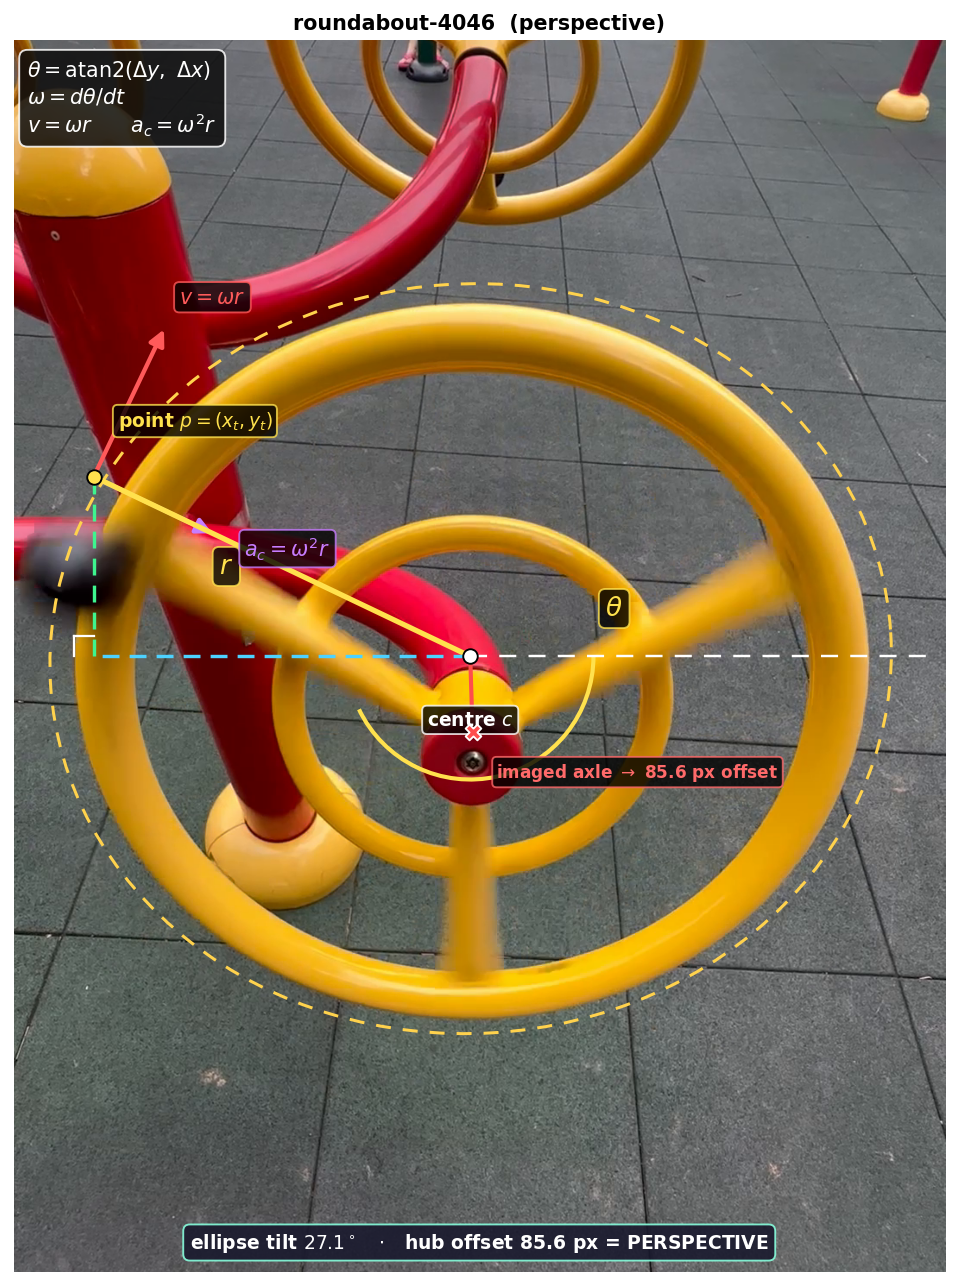
\includegraphics[width=0.72\linewidth]{fig-frame-4046.png}
\caption{The formulas of \S\ref{sec:howcomputed} on \texttt{roundabout-4046}. Centre $c$ and tracked
knob $p$ define the right triangle whose inverse tangent is $\theta=\operatorname{atan2}(\Delta y,
\Delta x)$; $r$, $v=\omega r$ (tangent) and $a_c=\omega^2 r$ (toward $c$) follow. The dashed ellipse
is the fitted orbit; the red $\times$ is the imaged axle, $85.6$\,px below the ellipse centre --- the
perspective offset this clip carries.}
\label{fig:frame4046}
\end{figure}

\textbf{Found.} A clean track (100\% coverage, zero jumps, area CV 0.23) carrying a large
artifact. The orbit is an ellipse (axis ratio 1.124, implied tilt $27.1^\circ$) and $94\%$ of
the $\omega$ ripple is phase-locked. The fingerprint is mixed ($A_1{=}1.594$, $A_2{=}0.657$,
ratio 2.43): perspective, not tilt.

The radius corroborates independently: the 2/rev component of $r(t)$ is $26.4$\,px, matching
the fitted ellipse's $(A-B)/2 = 26.9$\,px almost exactly, while its 1/rev component is only
$2.8$\,px --- so \textbf{the rotation centre is correct}, and the dominant 1/rev term in
$\omega$ is not a centring error.

\textbf{Improved.} Projective rectification (\S\ref{sec:method-rect}) reduced the ripple CV
from $0.166$ to $0.015$ and the 1/rev amplitude from $1.725$ to $0.054$
(Table~\ref{tab:rect}, Figure~\ref{fig:rectify}). This is the only clip in the corpus with a
\emph{measured} improvement; everything else in this report is diagnosis.

\begin{table}[htbp]
\centering
\footnotesize
\begin{tabular}{lrrr}
\toprule
Metric & Baseline & + drift removed & + projective rectified \\
\midrule
ripple CV                & 0.166 & 0.164 & \textbf{0.015} \\
$A_1$ (1/rev amplitude)  & 1.725 & 1.727 & \textbf{0.054} \\
$A_2$ (2/rev amplitude)  & 0.843 & 0.844 & \textbf{0.069} \\
phase-lock fraction      & 0.942 & 0.976 & \textbf{0.304} \\
orbit radial residual    & 5.20\% & --- & \textbf{1.68\%} \\
mean $|\omega|$ (rad/s)  & 7.799 & 7.799 & \textbf{7.800} \\
\bottomrule
\end{tabular}
\caption{Rectification on \texttt{roundabout-4046}. The baseline is deliberately generous: the
\emph{best least-squares circle} (not the sidecar's mark) plus the pipeline's exact
Savitzky--Golay${+}$median smoothing. The gain is therefore attributable to geometry, not to a
weakened baseline.}
\label{tab:rect}
\end{table}

\begin{figure}[htbp]
\centering
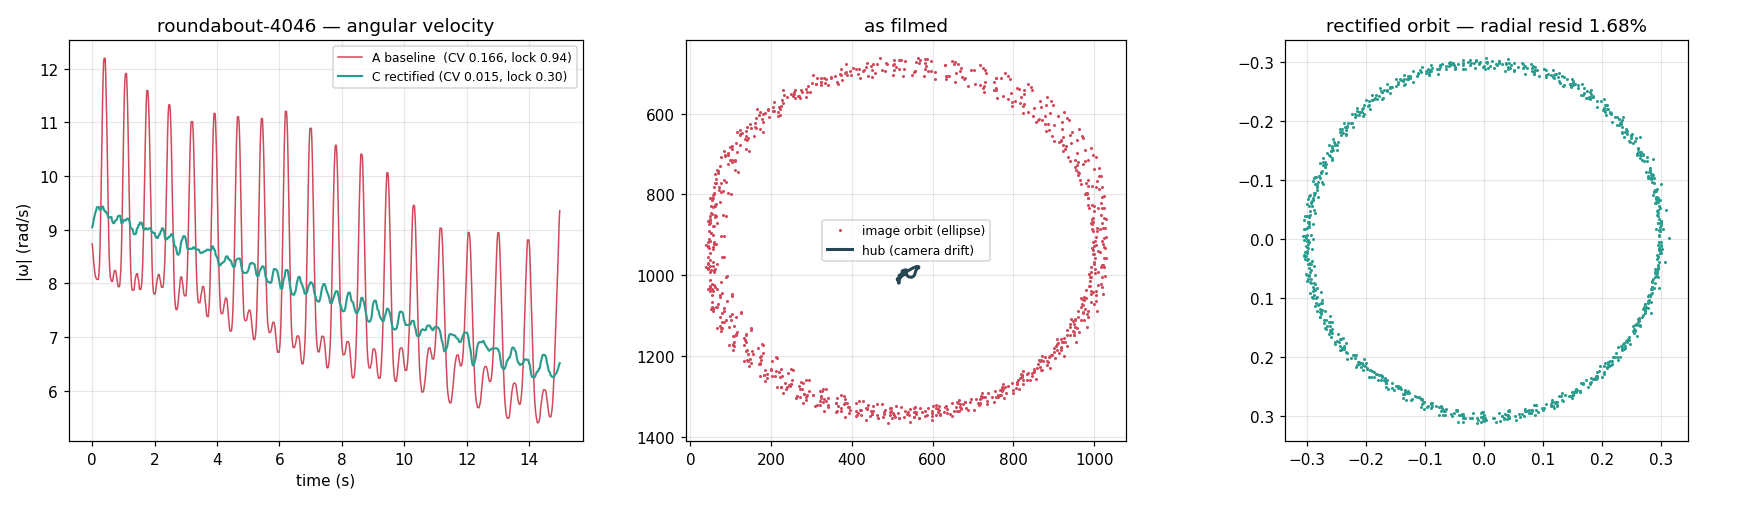
\includegraphics[width=\linewidth]{fig-rectify-4046.png}
\caption{\textbf{Left:} $\omega(t)$ as the pipeline produces it today (red) versus after
projective rectification (green). The red curve's $\sim$18 oscillations are a projection
artifact; the wheel simply coasts from 9.4 to 6.5\,rad/s. \textbf{Centre:} the orbit as filmed
--- a visible ellipse --- with the tracked hub showing $53\times41$\,px of handheld camera
drift. \textbf{Right:} the rectified orbit, now a circle to within 1.68\%.}
\label{fig:rectify}
\end{figure}

\textbf{Verdict: GOLD (corrected).} A real perspective artifact, removed by rectification with mean
$\omega$ invariant --- the one clip in the corpus that needed its \emph{data} corrected.

\subsection{bicycle --- phase-locked, but not perspective (unexplained)}

\textbf{Scene.} A phone threaded through the rear-wheel spokes of a bicycle on a stand --- the wheel
\emph{vertical} --- spun by hand and coasting down.

\textbf{Context handed to the agent.} Sidecar: \texttt{tracking\_mode: object} (SAM3), cue
\texttt{"red object"}, reference \texttt{"rear bicycle tire"} with \textbf{no
\texttt{physical\_size}} ($\Rightarrow$ the agent \emph{estimates} metres; \S\ref{sec:scale}),
\texttt{rotation\_center\_frac} $[0.340,0.655]$. \texttt{hints.md}: a phone threaded through the
rear-wheel spokes, the wheel vertical, spun by hand and coasting.

\textbf{How it is calculated.} The same trigonometric core: SAM3 gives the phone centroid, the
inverse-tangent angle of Eq.~2 turns it into orbital phase, and Savitzky--Golay differentiation gives
$\omega$. Because the wheel is \emph{vertical}, gravity is a candidate 1/rev driver, so besides the
phase-harmonic regression ($A_1{=}0.846$, $A_2{=}0.286$) the ripple's peak phase is compared against
bottom-of-swing (it lands $138^\circ$ away --- wrong for gravity). Periodic occlusion is tested by
\textbf{regressing the phone's visible mask area on orbital phase} ($R^2{=}0.073$). Scale --- absent
from the sidecar --- is estimated by using the phone's \textbf{rotation-invariant oriented bounding
box} (long side $123.9$\,px) as a known-length ruler against the tracked tire (\S\ref{sec:scale}).

\begin{figure}[htbp]
\centering
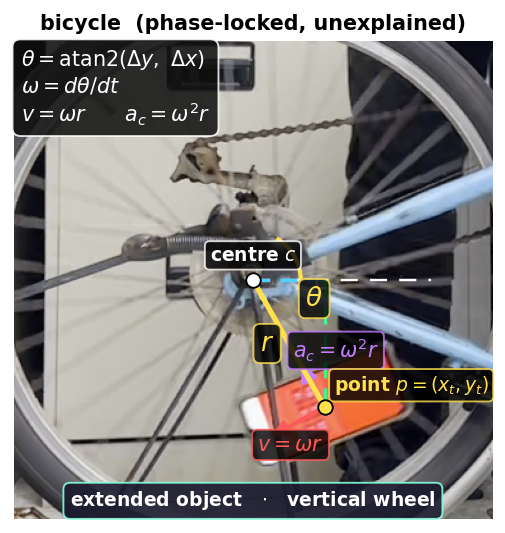
\includegraphics[width=0.72\linewidth]{fig-frame-bicycle.png}
\caption{The formulas of \S\ref{sec:howcomputed} on \texttt{bicycle}: centre $c$ at the wheel hub,
tracked point $p$ on the phone threaded through the spokes, and the $\theta$/$r$/$v$/$a_c$ geometry.
The target is an \emph{extended} object on a \emph{vertical} wheel --- the two features behind the
unexplained phase-locked ripple.}
\label{fig:framebicycle}
\end{figure}
tracked correctly throughout (100\% coverage, zero jumps). Tilt $15.0^\circ$, 6.4 revolutions.
Its ripple \emph{is} phase-locked ($0.72$) with a 1/rev-dominant fingerprint
($A_1{=}0.846$, $A_2{=}0.286$) --- the signature that an earlier draft read as perspective.

\textbf{It is not perspective.} The imaged hub was detected in 90\% of frames and verified on
frames; it sits only $4.9$\,px from the centre of the elliptical path. Under an affine view
those points coincide, so a $4.9$\,px offset means the projection is essentially affine and
there is no perspective to undo. Rectification confirms it: ripple CV $0.141 \to 0.148$ and
the radial residual \emph{worsens} ($3.94\% \to 4.47\%$).

\textbf{It is not occlusion either.} The phone passes behind the frame and derailleur once per
revolution, which would cut the mask and shift its centroid. Tested and rejected: visible area
against orbital phase gives $R^2 = 0.073$, with a 1/rev amplitude of only 5.9\% of mean area.

\textbf{Cause unknown.} The clip tracks an \emph{extended} object rather than a near-point
marker, so a shape-dependent centroid effect is the leading hypothesis --- but it is untested
and is not claimed here. Note also that $0.72$ over 6.4 revolutions is weaker evidence than
4046's $0.94$ over 18.6; part of it may be the phase-lock statistic's own variance.

\textbf{Improved.} Nothing. This clip is an open problem, and the honest reading is that we do
not yet know what its data should look like.

\subsubsection*{A scale cross-check that fails --- and why it is not the blocker}
\label{sec:scale}

Scale is \emph{not} why this clip fails. $\omega$, $T$ and $f$ are \textbf{scale-free} (pure
angle over time; \texttt{px\_per\_m} never enters), and bicycle fails on its $\omega$ ripple. A
perfect scale would leave that ripple byte-for-byte identical. Scale reaches only $v = \omega r$
and $a_c = \omega^2 r$.

That said, this clip's sidecar carries \textbf{no \texttt{physical\_size} at all} --- only
\texttt{label: "rear bicycle tire"} and a bbox centre. Per the data contract, absent means
\emph{the agent estimates it}: bicycle's metres are currently guessed.

Using the tracked phone as a known-size reference (its oriented box is rotation-invariant: long
side 123.9\,px, CV 0.021, better than the axis-aligned bbox's 0.034) against the tracked tire
(outer diameter 484\,px):

\begin{center}
\begin{tabular}{lrr}
\toprule
assumed phone body length & $\rightarrow$ px/m & $\rightarrow$ derived tire diameter \\
\midrule
140\,mm (the 5.5$''$ \emph{screen diagonal} --- wrong dimension) & 885 & 54.7\,cm \\
\textbf{150\,mm} (typical 5.5$''$ body) & 826 & \textbf{58.6\,cm} \\
158\,mm & 784 & 61.7\,cm \\
\bottomrule
\end{tabular}
\end{center}

A real wheel is \textbf{66--70\,cm} outer (26$''$ MTB $\approx$ 66, 700c $\approx$ 68). Inverting:
a standard 66\,cm wheel demands a \textbf{169\,mm} phone body --- a large phone, not a 5.5$''$ one.
\textbf{Two independent references disagree by ${\sim}12\%$, so one is wrong.} The prime suspect is
that the phone is threaded \emph{through} the spokes, so they occlude it and the mask --- hence the
obox --- is systematically short. That is independent evidence the phone's mask is unclean, which
is suggestive for the unexplained ripple without confirming it.

\textbf{Trap:} ``5.5 inch'' is a \emph{screen diagonal}, not a physical edge; the obox long side
measures the phone's \emph{body length}. Confusing them is a ${\sim}7\%$ error straight into $v$
and $a_c$. Settle it with a ruler on the phone body and the wheel.

\textbf{Verdict: OPEN.} A phase-locked ripple that is neither perspective nor occlusion (cause
unknown), on a clip whose scale is also only estimated --- we cannot yet say what its data should be.

\subsection{turntable-1 --- no artifact; the data is already right}

\textbf{Scene.} A red phone on a black turntable, filmed from above; a spin that coasts down.

\textbf{Context handed to the agent.} Sidecar: \texttt{tracking\_mode: object} (SAM3), cue
\texttt{"red phone"}, reference \texttt{"black circular base"} (\texttt{physical\_size: 0.4}\,m),
\texttt{rotation\_center\_frac} $[0.526,0.428]$. \texttt{hints.md}: a red phone on a black turntable,
filmed from above; verified frame-by-frame that the tracker locks the phone throughout.

\textbf{How it is calculated.} Identical chain --- SAM3 centroid, the inverse-tangent angle of Eq.~2,
then Savitzky--Golay $\omega$. The decisive quantity here is the \textbf{phase-lock fraction}: the
share of ripple variance the phase-harmonic regression explains is only $0.15$, i.e.\ the ripple is
broadband detector noise, not a geometric artifact. The bright spindle is located by
\textbf{brightness/HSV thresholding} and sits just $8.8$\,px from the ellipse centre, so the raw
inverse-tangent angle is already correct and no rectification is applied.

\begin{figure}[htbp]
\centering
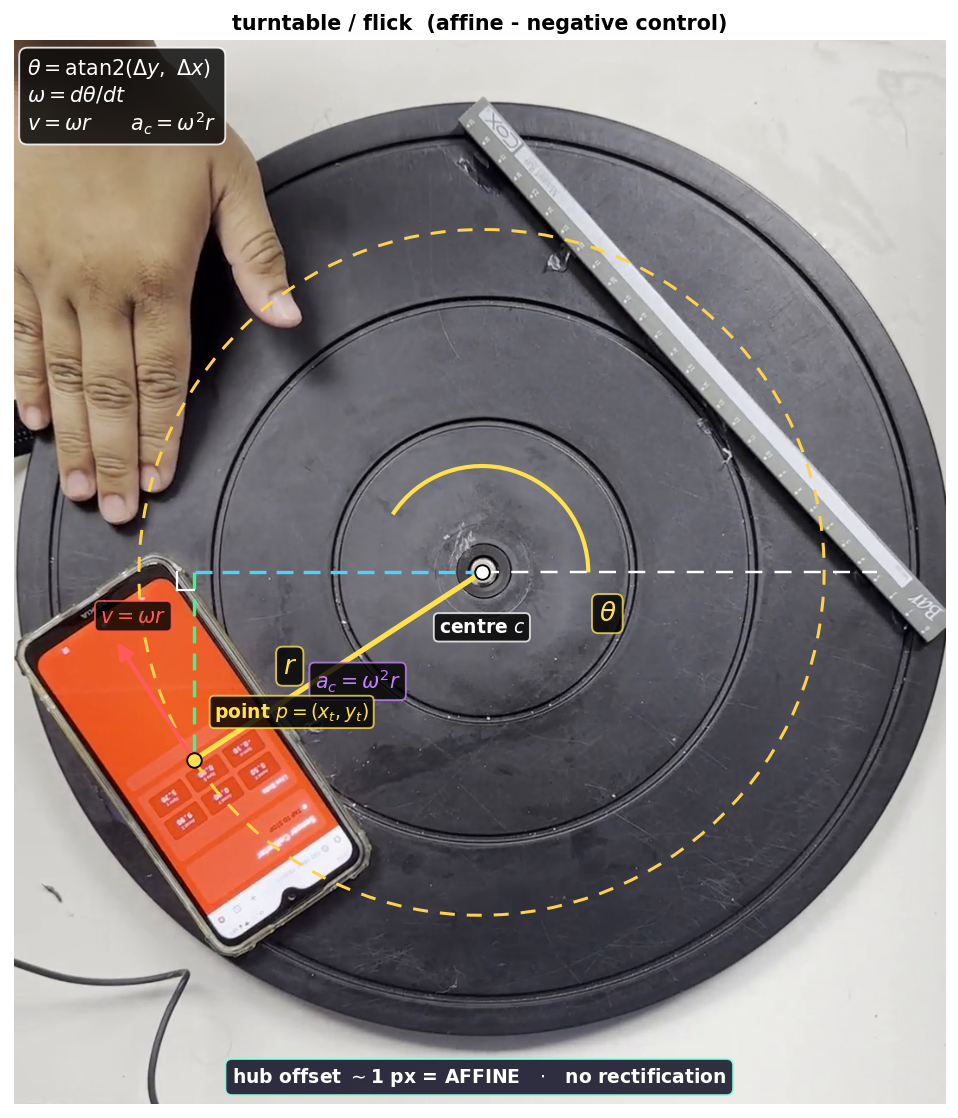
\includegraphics[width=0.72\linewidth]{fig-frame-turntable.png}
\caption{The formulas of \S\ref{sec:howcomputed} on the turntable (\texttt{flick}): centre $c$ at the
spindle, tracked point $p$ on the phone. The fitted orbit is nearly circular and the spindle sits
$\sim$1\,px from its centre --- an \emph{affine} view, so $\theta=\operatorname{atan2}(\Delta y,
\Delta x)$ is already correct and rectification is (correctly) withheld.}
\label{fig:frameturntable}
\end{figure}

\textbf{Found.} Track verified clean on frames (Figure~\ref{fig:turntable1}): the crosshair sits
on the phone in every sampled frame and the platter is visibly elliptical ($14.9^\circ$).

\textbf{But the ellipse is affine, and the ripple is not an artifact.} The bright metallic
spindle at the platter centre was detected in \textbf{100\%} of frames and lies $8.8$\,px from
the centre of the elliptical path --- essentially coincident. Correspondingly the ripple is
\textbf{not phase-locked at all} (lock $= 0.15$ over 2.6 revolutions): its ripple CV of $0.159$
is broadband detector noise, not geometry. An earlier draft classified this clip as
``perspective'' purely from its $A_1/A_2$ ratio; \S\ref{sec:null} retracts that.

\textbf{Improved.} Nothing, and nothing is needed --- which makes this clip valuable. It is a
\emph{negative control}: a tilted clip whose $\theta$ is already correct, and on which
rectification measurably must not fire. Rectification leaves it unchanged
($0.159 \to 0.162$), as required.

\begin{figure}[htbp]
\centering
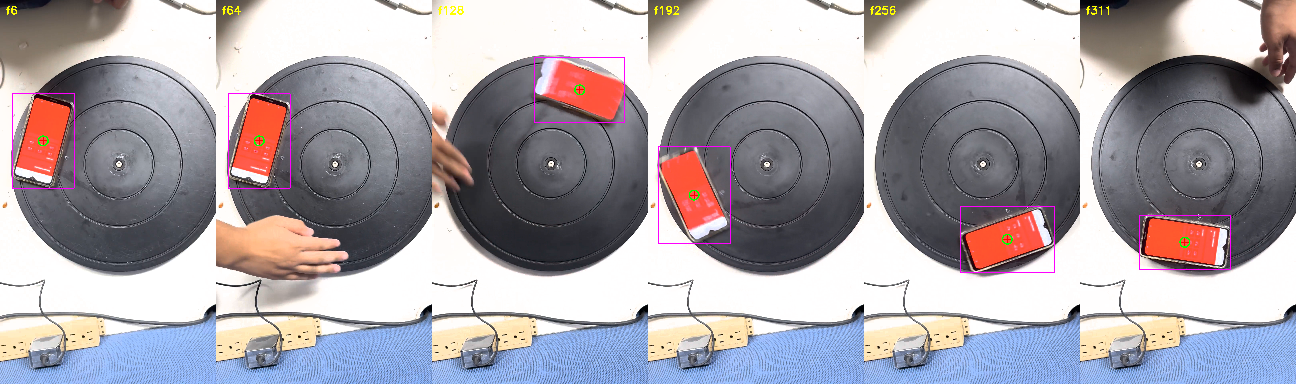
\includegraphics[width=\linewidth]{fig-track-turntable1.png}
\caption{\texttt{turntable-1}: detection verified. The crosshair tracks the phone across the
clip and the box follows its rotation. The elliptical rim is the $14.9^\circ$ tilt --- but the
imaged spindle sits only 8.8\,px from the ellipse centre, so that tilt is an \emph{affine} view
and $\theta$ needs no correction.}
\label{fig:turntable1}
\end{figure}

\textbf{Verdict: GOLD (as-is).} A negative control: tilted $14.9^\circ$ yet affine, so $\theta$ is
already correct and a gate must provably \emph{not} fire on it.

\subsection{turntable-2, turntable-3 / flick --- undecidable, not clean}

\textbf{Scene.} A red phone on a black circular base, filmed nearly top-down: at rest, one flick
($t\approx2.1$\,s), then a coast to a stop.

\textbf{Context handed to the agent.} Both carry the turntable sidecar: \texttt{tracking\_mode:
object}, cue \texttt{"red phone"}, reference \texttt{"black circular base"}
(\texttt{physical\_size: 0.4}\,m). The marked \texttt{rotation\_center\_frac} is $[0.515,0.419]$
(t-2) and $[0.503,0.457]$ (t-3\,$=$\,flick). \texttt{flick}'s \texttt{hints.md} flags it as the golden
template (job \texttt{9ed918d0}): rest, one flick at $t{\approx}2.1$\,s, then coast-down.

\textbf{How it is calculated.} Same trigonometric angle (Eq.~2) and Savitzky--Golay
$\omega$. The difference is coverage: the harmonic fingerprint needs $\ge 2$ revolutions to separate
$A_1$ from $A_2$, and these clips give only $1.4$ and $1.8$ --- so the fingerprint is left undefined
and they are reported \und{}. The \textbf{hub offset}, a \emph{static} measurement (imaged spindle vs
ellipse centre, needing no revolutions), still applies: $3.4$ and $0.7$\,px $\Rightarrow$ no
perspective. Near face-on (axis ratio $1.002$) the conic axes are ill-conditioned, so rectification
is deliberately withheld.

\textbf{Found.} Both tracks are clean. Both are \emph{too short to diagnose}: 1.4 and 1.8
revolutions of active motion against a floor of 2. Their tilts are real ($11.3^\circ$ and
$3.8^\circ$) but their $A_1/A_2$ cannot be separated.

This distinction matters and is easy to lose: \textbf{\und{} is not a clean bill of health.}
\texttt{turntable-3}/\texttt{flick} is the least-tilted clip in the corpus at $3.8^\circ$ and
the closest thing we have to a well-captured example --- but ``least tilted'' is not
``untilted'', and its apparent quality was decided by the tripod, not by processing.

\textbf{Improved.} Nothing, and rectification must \textbf{not} be applied: at an axis ratio of
1.002 the conic's axes are ill-conditioned, the vanishing line is numerically unstable, and
rectifying would inject error rather than remove it. Near face-on, leave the geometry alone.

\textbf{Verdict: GOLD (as-is).} Undecidable by fingerprint (under two revolutions), but cleared of
perspective by the static hub offset; near face-on, the geometry is left untouched.

\subsection{fan-4027, fan-4028 --- the synth fabricates the ends; measurement makes them SILVER}
\label{sec:fans}

\textbf{Scene.} A five-blade ceiling fan with a red-paper marker on one blade tip; two-phase motion
--- spins up to a peak, then coasts to rest.

\textbf{Context handed to the agent.} Sidecar: \texttt{tracking\_mode: frequency}; cue
\texttt{"fan blade"}; \texttt{rotation\_center\_frac} $[0.5271,0.4444]$ (the hub, $\approx(1012,480)$
px); \texttt{tracking\_config} $\{$\texttt{n\_blades: 5}, \texttt{ring\_radius: 180},
\texttt{orbit\_radius\_px: 355}, \texttt{n\_probes: 12}, \texttt{window\_s: 2.5},
\texttt{hop\_s: 0.5}$\}$; reference \texttt{"blade-tip orbit"} with \texttt{physical\_size: 0.635}
(the ruler-measured tip radius, below). The injected \texttt{hints.md} states plainly that the
orbit is \emph{synthesized} and must never be presented as a measured trajectory --- the standing
caveat that makes these clips SILVER rather than GOLD (\S\ref{sec:golden}).

\textbf{How it is calculated (different in kind).} Unlike every clip above, movement here is
\emph{not} read by trigonometry on a tracked point --- a motion-blurred rotor of five identical blades
exposes no point to apply $\operatorname{atan2}$ to. Instead image intensity is sampled at a ring of
probes around the hub; each blade sweeping past a probe dips that signal, and a \textbf{windowed FFT}
of it gives the blade-pass frequency $f_b$. With $N{=}5$ blades the rotation rate is
\[
  \omega \;=\; 2\pi\,\frac{f_b}{N}
\]
(Eq.~6). The per-frame angle and orbit are then \emph{synthesized} from $\omega$, not measured ---
the root of the SILVER caveat. Scale comes from the calibration ratio (Eq.~1), and the tip speed and
centripetal acceleration (Eq.~4) are evaluated at the ruler-measured blade-tip radius.

\textbf{Found.} These clips ship \texttt{tracking\_mode: frequency}: \texttt{freq\_track} recovers
$\omega$ from blade-pass frequency and then \emph{generates} a circular orbit from it. The
signatures are values no real capture produces --- axis ratio exactly $1.000$, box area CV exactly
$0.00$, centroid jitter $0.06$\,px.

\textbf{The mode was never justified for these clips.} The NOTES give the reason as \emph{``SAM3
aliases 5 identical blades''} --- an \textbf{identity} problem, not a speed one, and a unique
marker solves identity outright. There was never an aliasing risk either: at $\omega \approx
4$\,rad/s the marker moves ${\sim}17$\,px/frame $= \mathbf{8^\circ}$/frame, and blade-pass is
3.2\,Hz against a 30\,Hz Nyquist limit. The NOTES even record that the marker \emph{was}
colour-tracked to obtain the geometry (orbit CV 0.05) --- and the trajectory was synthesized anyway.

\textbf{What the synth gets wrong: it has a floor at 1.0\,rad/s.} Below the minimum detectable
blade-pass frequency it emits $1.0$\,rad/s regardless of the truth.

\begin{center}
\begin{tabular}{lrr}
\toprule
 & fan-4027 & fan-4028 \\
\midrule
measured $|\omega|$, first 2\,s & \textbf{0.002}\,rad/s (at rest) & \textbf{0.006}\,rad/s (at rest) \\
measured $|\omega|$, last 2\,s  & \textbf{0.070}\,rad/s (at rest) & \textbf{0.132}\,rad/s (at rest) \\
\textbf{synth, both ends}       & \textbf{1.004\,rad/s} & \textbf{1.004\,rad/s} \\
\bottomrule
\end{tabular}
\end{center}

\textbf{The synth claims the fan never stops.} 4027's own NOTES say it \emph{``coasts DOWN to rest
by ${\sim}t=60$\,s''}; the shipped curve holds $1.0$\,rad/s to $t=77$\,s (Figure~\ref{fig:fans}).
It was also a \textbf{staircase} --- one $\omega$ per FFT window, quantised to
$\Delta\omega \approx 0.5$\,rad/s by Eq.~\eqref{eq:quant} --- where the true motion is smooth. That
staircase is a pure method artifact (only \texttt{frequency} mode shows it; per-frame clips such as
\texttt{4029} and \texttt{flick} come out smooth), and it is now removed at source by sub-bin peak
interpolation (\S\ref{sec:howcomputed}; Figure~\ref{fig:fans}). It also draws a \textbf{perfect
circle} where the real orbit is a slight ellipse (axis 1.042).

\textbf{The pedagogical consequence is direct.} \texttt{material\_hints.md} instructs: \emph{never
say it ``comes to rest'' unless the data says it actually stopped in the clip}. With the synth the
fan never stops, so the material is compelled to write \emph{``still turning, only slower''} ---
\textbf{which is false}. The measured marker lets it tell the truth.

\textbf{The rate is independently verified.} Colour-tracking the red blade marker (predict-and-match
gating, step bound from $\omega r/\mathrm{fps}$) reproduces the blade-pass $\omega$ where both are in
range:

\begin{center}
\begin{tabular}{lrrrrl}
\toprule
 & coverage & revs & ripple CV & phase-lock & verdict \\
\midrule
fan-4027 & \textbf{100.0\%} & 22.6 & 0.084 & 0.121 & clean, no artifact \\
fan-4028 & \textbf{99.4\%} & 29.0 & \textbf{0.054} & 0.197 & clean --- \textbf{lowest ripple in the corpus} \\
\bottomrule
\end{tabular}
\end{center}

The two agree in range (correlation \textbf{0.974}; mean $\omega$ within 7.7\%), so the frequency
mode's \emph{rate} was right all along --- only the fabricated ends and the staircase were wrong. We
nonetheless \textbf{keep frequency mode as shipped}: it needs no per-frame point, whereas colour
tracking is defeated by motion blur at the $t{=}20$\,s peak ($\omega \approx 11.5$\,rad/s moves the
tip ${\sim}11$\,cm per frame). The colour track is a validation of the rate, not the delivered
trajectory.

\begin{figure}[htbp]
\centering
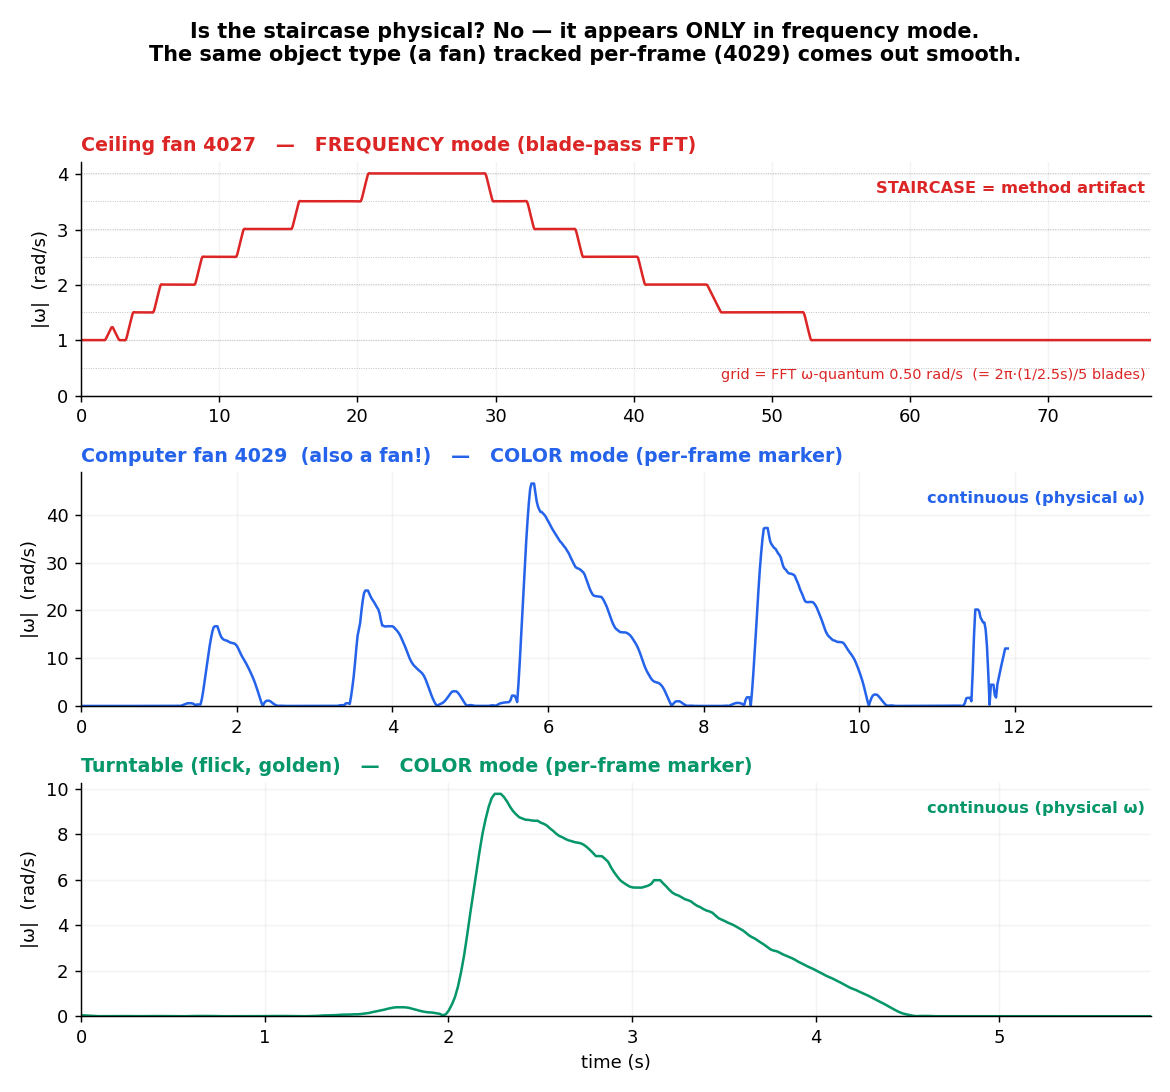
\includegraphics[width=\linewidth]{fig-fan-omega-method.png}
\caption{The staircase is a \emph{method} artifact, not the fan. \textbf{Top:} \texttt{fan-4027}
in \texttt{frequency} mode --- the raw FFT bin quantises $\omega$ onto a $0.5$\,rad/s grid
(Eq.~\eqref{eq:quant}, dotted). \textbf{Middle:} \texttt{computerfan-4029}, \emph{also a fan} but
colour-tracked per frame, comes out smooth. \textbf{Bottom:} the turntable (\texttt{flick}),
per-frame, likewise smooth. Only \texttt{frequency} mode staircases; the sub-bin parabolic fit
(\S\ref{sec:howcomputed}) recovers the smooth curve the steps were quantising.}
\label{fig:fanmethod}
\end{figure}

\begin{figure}[htbp]
\centering
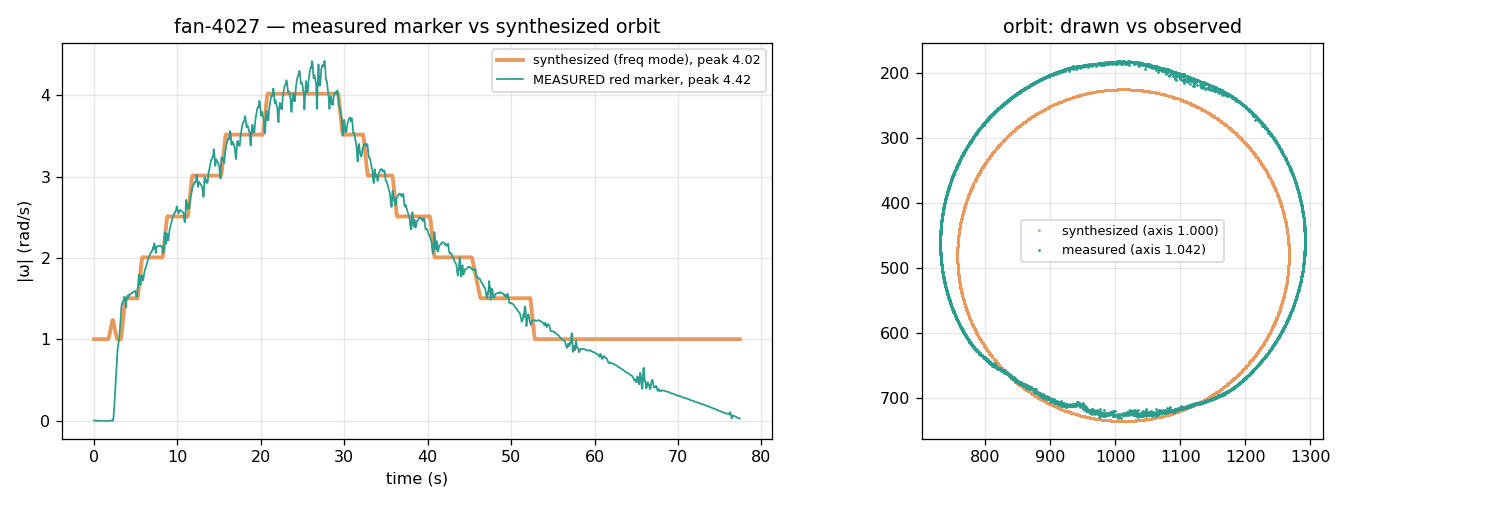
\includegraphics[width=\linewidth]{fig-fan-synth-vs-measured.png}
\caption{\texttt{fan-4027}, \emph{diagnosis (pre-fix)}: the shipped \texttt{frequency} curve
(orange) against the measured red blade marker (green). The synth is a staircase, and it
\textbf{flatlines at 1.0\,rad/s from $t{=}57$\,s} while the fan is visibly coasting to a stop ---
and again at $t{=}0$--$3$\,s while at rest. \textbf{Right:} the drawn orbit (a perfect circle)
against the observed one (a slight ellipse). The staircase (Eq.~\eqref{eq:quant}) is since removed
by sub-bin interpolation (Figure~\ref{fig:fanmethod}) and the scale measured at $559$\,px/m.}
\label{fig:fans}
\end{figure}

\textbf{A sticky-error bug, re-committed in our own tracker.} 4028 first gave 46.7\% coverage,
collapsing to 0\% from $t=50$\,s --- \emph{not} motion blur (coverage is 100\% through the
$t=20$\,s peak). Our predict-and-match gate had gone \textbf{sticky}: once \texttt{prev} was wrong,
every candidate was rejected forever. That is verbatim the \texttt{roundabout-4048} defect this
report documents (\S\ref{sec:4048bugs}), reproduced by us. Adding re-acquisition after 0.4\,s of
loss took it to \textbf{99.4\%}, with \emph{zero} contiguous teleports (worst consecutive step
$22^\circ$/frame at peak); every large step spans a detection gap.

\textbf{Scale --- measured (resolved).} A ruler settles the last open quantity. Hub-to-blade-tip
$=63.5$\,cm (a $25''$ fan), blade length $20''$; the blade tip images at $355$\,px (sd $0.5$ over
frames), so by Eq.~\eqref{eq:calib}
\[
\mathrm{px\_per\_m} \;=\; \frac{355\ \mathrm{px}}{0.635\ \mathrm{m}} \;=\; 559\ \mathrm{px/m},
\]
retiring the provisional \texttt{physical\_size: 0.6} (which had implied $425$\,px/m, a $31\%$ scale
error). The sidecars now pin both \texttt{orbit\_radius\_px} and \texttt{physical\_size} to the blade
tip ($355$\,px $/\,0.635$\,m), so $v$ and $a_c$ are reported \textbf{at the blade tip} --- the
student-natural maximum. This is exact, not extrapolation: $\omega$ is rigid-body and comes from the
blade-pass FFT rather than the marker, so both inputs to the linear-speed relation (Eq.~4) --- the
rate $\omega$ and the tip radius --- are measured. Evaluated at the peak $\omega$:

\begin{center}
\begin{tabular}{lrrr}
\toprule
 & peak $|\omega|$ (rad/s) & $v_{\mathrm{tip}} = \omega r$ & $a_c = \omega^2 r$ \\
\midrule
fan-4027 & 4.21 & $2.68$\,m/s ($9.6$\,km/h) & $\mathbf{11.3}$\,m/s$^2$ ($1.15\,g$) \\
fan-4028 & 11.59 & $7.36$\,m/s ($26.5$\,km/h) & $\mathbf{85.2}$\,m/s$^2$ ($8.69\,g$) \\
\bottomrule
\end{tabular}
\end{center}

The tracked marker itself orbits inboard at ${\sim}49$\,cm, so switching to
\texttt{tracking\_mode: color} is \emph{not} needed for $v$/$a_c$. Verified end-to-end through the
real \texttt{analysis.run} ($\mathrm{px\_per\_m}=559$, $r_{\mathrm{fit}}=0.635$\,m) with the
pipeline's unit tests passing.

\begin{figure}[htbp]
\centering
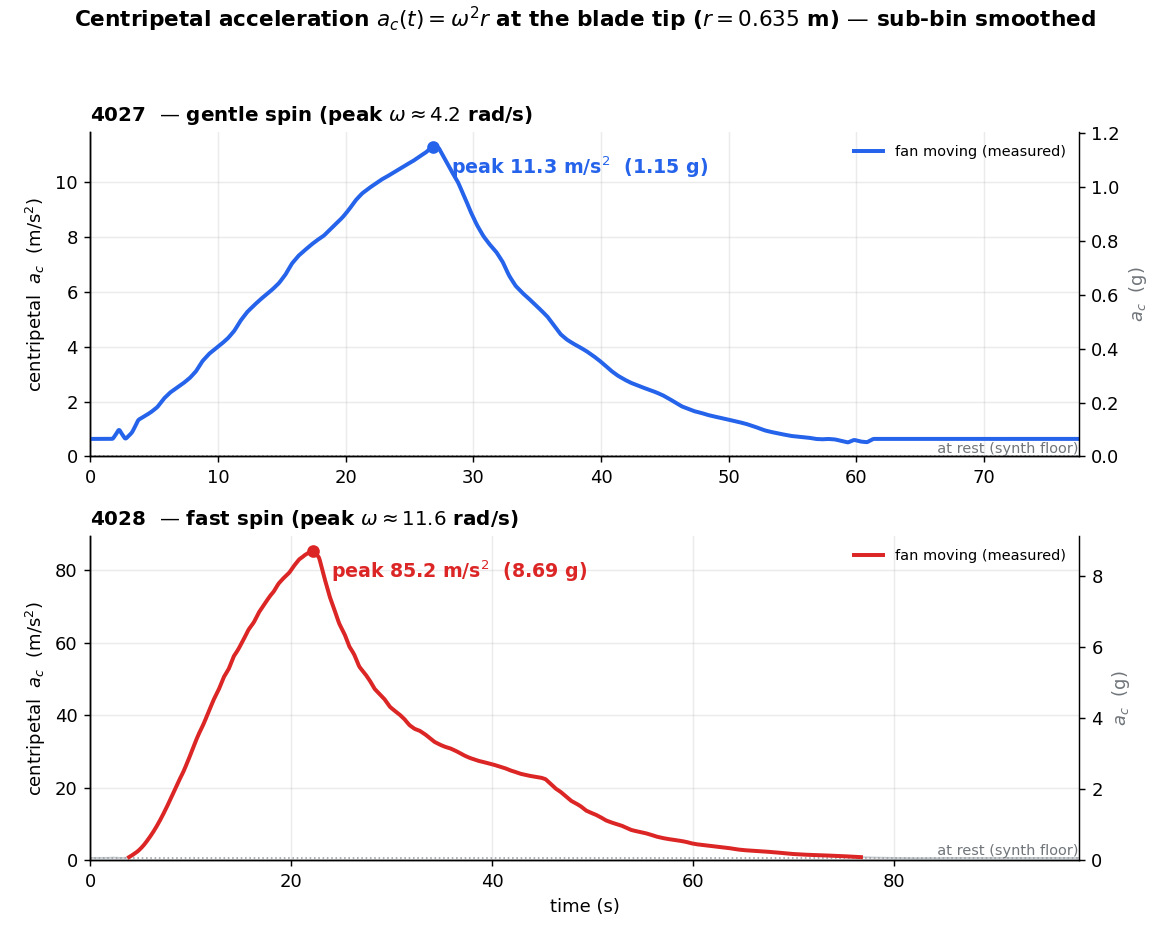
\includegraphics[width=\linewidth]{fig-fan-ac-t.png}
\caption{Centripetal acceleration $a_c(t) = \omega^2 r$ at the blade tip ($r=0.635$\,m), after
sub-bin smoothing --- the student-facing curve. Both fans show a smooth spin-up to a peak and a
coast-down, as a real rotor does. \textbf{Top:} \texttt{fan-4027}, peak $11.3$\,m/s$^2$ ($1.15\,g$).
\textbf{Bottom:} \texttt{fan-4028}, peak $85.2$\,m/s$^2$ ($8.69\,g$) --- the tip pulls over $8\times$
gravity. The dotted floor is the synth's residual reading while the fan is at rest (marked, not
shown as motion).}
\label{fig:fanact}
\end{figure}

\textbf{Verdict: SILVER.} The rate ($\omega$, $T$, $f$) and now the scale ($v$, $a_c$) are measured
and teachable, but the per-frame \emph{trajectory} is reconstructed from the rate, not observed: a
blurred, identical-blade rotor exposes no resolvable point to track. Teach the numbers freely;
present the orbit as a model, never as measured data (\S\ref{sec:golden}).

\subsection{computerfan-4029 --- clean; our own gate accused it falsely}
\label{sec:4029}

\textbf{Scene.} A red marker on a PC case-fan blade, spun by hand in short bursts.

\textbf{Context handed to the agent.} Sidecar: \texttt{tracking\_mode: color}, cue
\texttt{"red marker"}, reference \texttt{"red marker"} (\texttt{physical\_size: 0.04}\,m),
\texttt{rotation\_center\_frac} $[0.519,0.473]$, \texttt{tracking\_config} $\{$\texttt{hsv\_lo}
$[168,80,80]$, \texttt{hsv\_hi} $[12,255,255]$ (red wraps the hue origin, $168\to12$),
\texttt{roi\_radius: 520}, \texttt{max\_step: 300}, \texttt{min\_area: 100}$\}$. \texttt{hints.md}:
a red marker on a PC case-fan blade, hand-spun in bursts.

\textbf{How it is calculated.} \texttt{color} mode thresholds the red marker in HSV (the config's
$168\to12$ hue wrap spans red across the origin) to a per-frame centroid, then the same
inverse-tangent angle (Eq.~2) and Savitzky--Golay $\omega$. What matters here is the \textbf{gate}
that flagged it: a frame-to-frame pixel step counts as a teleport only if it exceeds the physical
expectation for a correctly-tracked point,
\[
  \text{expected step} \;=\; \frac{\omega\, r}{\mathrm{fps}} \quad [\mathrm{px/frame}].
\]
At $r{=}312$\,px and $4$\,rev/s this is $131$\,px --- so the $153$ ``jumps'' are real motion, not
teleports. The equivalent angular step $\omega/\mathrm{fps}$ peaks at $55^\circ$, far below the
$180^\circ$ aliasing limit, and all statistics are restricted to the active burst
($6.7$ revolutions).

\begin{figure}[htbp]
\centering
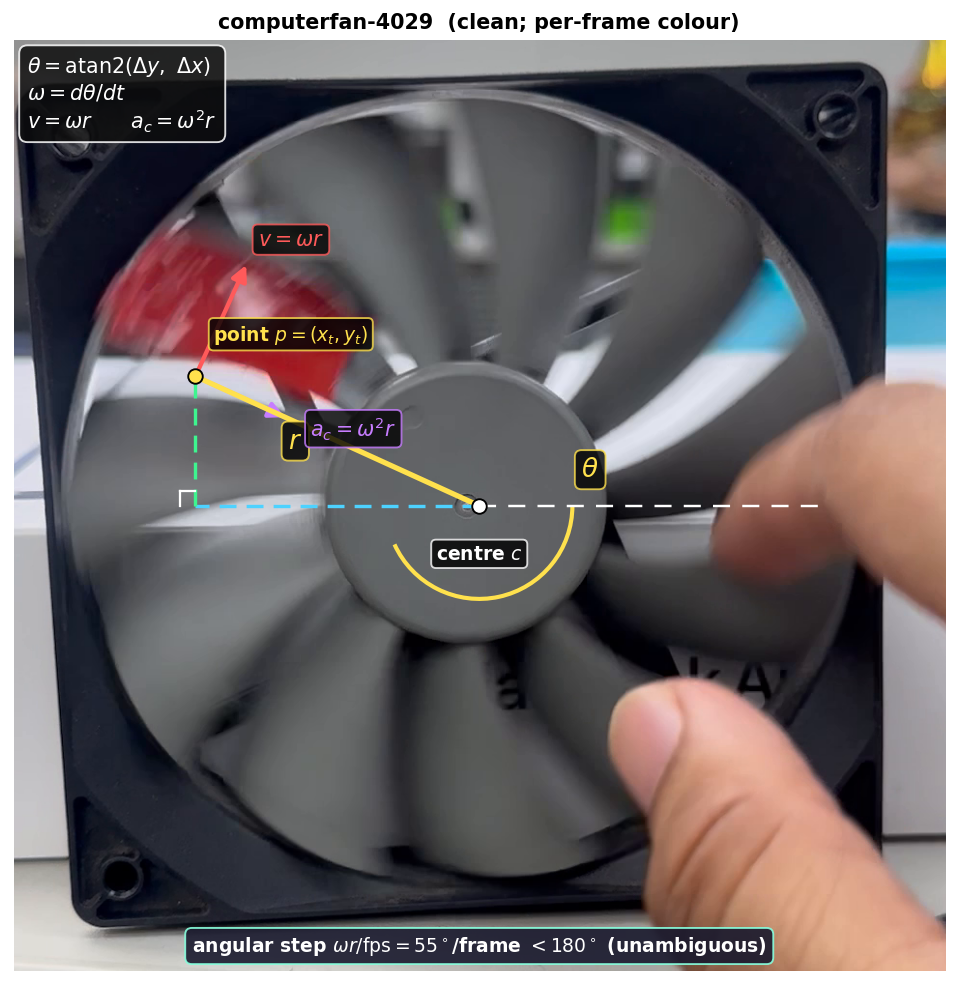
\includegraphics[width=0.72\linewidth]{fig-frame-4029.png}
\caption{The formulas of \S\ref{sec:howcomputed} on \texttt{computerfan-4029}: centre $c$ at the fan
hub, tracked point $p$ on the red blade marker (\texttt{color} mode, per frame). The angular step
$\omega r/\mathrm{fps}=55^\circ$ stays well below the $180^\circ$ aliasing limit, so the
$131$\,px pixel steps are real $4$\,rev/s motion --- not the teleports the fixed-pixel gate alleged.}
\label{fig:frame4029}
\end{figure} Coverage 86.9\%, ``153 steps over 100\,px'', step p99 of
268.9\,px against a median of 6.7\,px. The gate called it \susp{} and an earlier draft of this
report repeated that as ``contaminated''.

\textbf{Found (after looking).} The track is \emph{correct}. Every sampled frame has the
crosshair on the red blade marker. Two facts dissolve the accusation:

\begin{itemize}
  \item \textbf{The missing 13\% is one contiguous run} (\texttt{f717--824}, $t = 11.96$--$13.74$\,s)
  where the shot pans off the fan entirely. That is honest absence, not failed detection.
  \item \textbf{The ``153 teleports'' are real motion.} The fan is spun in \emph{bursts} --- the
  per-second median step swings from 0.1\,px (at rest) to 133\,px (4.08\,rev/s). At $r = 312$\,px,
  4\,rev/s \emph{is} 131\,px/frame. The angular step peaks at $55^\circ$/frame, far below the
  $180^\circ$ aliasing limit, so the trajectory is unambiguous throughout.
\end{itemize}

\textbf{Diagnosis.} Restricted to the largest burst (1.53\,s, \textbf{6.7 revolutions} --- ample
phase coverage), with the fan's grey centre boss detected in \textbf{99.4\%} of frames and
verified on frames:

\begin{center}
\begin{tabular}{lr}
\toprule
Hub offset & \textbf{8.5\,px} $\Rightarrow$ no perspective \\
Axis ratio / tilt & 1.021 / $11.8^\circ$ \\
Mean $|\omega|$ & 27.89\,rad/s \\
Ripple CV & \textbf{0.088} --- the lowest of any real clip in the corpus \\
Phase-lock & \textbf{0.075} $\Rightarrow$ no artifact \\
\bottomrule
\end{tabular}
\end{center}

\textbf{Improved.} The clip needs no geometric correction: its data is already right. The
earlier ``axis ratio 1.075 / $21.5^\circ$ tilt'' was a conic fitted to the whole clip including
the pan-away; restricted to the burst it is $11.8^\circ$. \textbf{This is the third phenomenon
whose data we can vouch for}, and it was recovered by fixing our diagnostic, not the clip.

\textbf{The lesson is about the gate, not the fan.} A fixed pixel threshold encodes an
assumption about speed that no clip is obliged to honour. It is the same error family as the
rest of this report: a statistic applied without asking what the scene is physically doing.

\textbf{Verdict: GOLD (as-is).} The \susp{} flag was our own gate's false positive; the track is
clean and needs no correction --- recovered by fixing the diagnostic, not the clip.

\subsection{fan-doll --- detection fails on both backends (rejected)}
\label{sec:fandoll}

\textbf{Scene.} A cream plush toy with a small green sprout on top, tied to one blade of a ceiling
fan and filmed against a cream ceiling.

\textbf{Context handed to the agent.} Sidecar: \texttt{tracking\_mode: object} (SAM3), cue
\texttt{"yellow toy"}, reference \texttt{"fan blade"} (\texttt{physical\_size: 0.32}\,m),
\texttt{rotation\_center\_frac} $[0.579,0.503]$. \texttt{hints.md} opens with the verdict itself:
\emph{NOT usable as filmed --- report \texttt{failed}, do not produce material}.

\textbf{How it is calculated (why it cannot be).} No angle is computed: the cue \texttt{"fan blade"}
matched the window louvres and \texttt{"yellow toy"} returned nothing, so there is no trajectory to
feed Eq.~2. The recovery attempt is an \textbf{HSV separability test} on the toy's green sprout
($S=98$--$161$ against a ceiling $S\approx20$); colour-tracking it reaches $51.7\%$ coverage, but the
sprout rotates out of view (box-area CV $1.30$), so no usable $\omega$ results.

\begin{figure}[htbp]
\centering
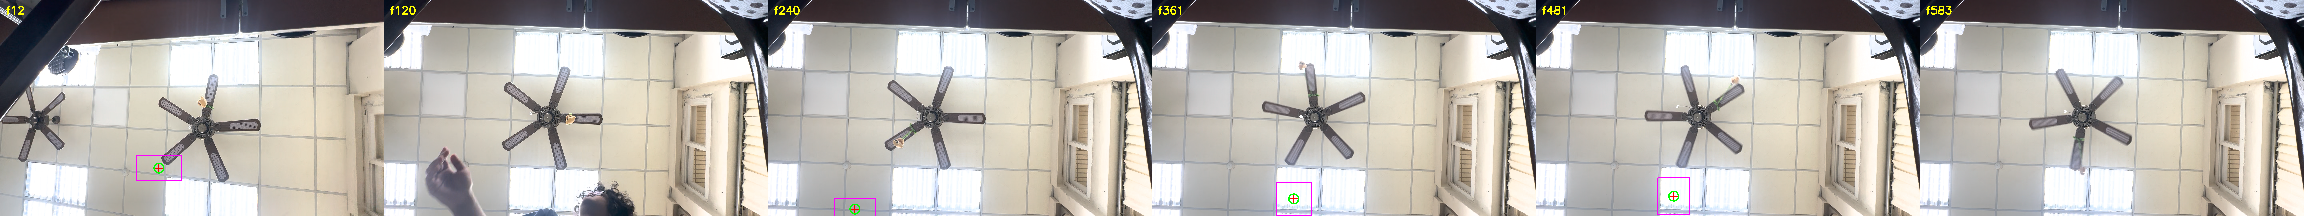
\includegraphics[width=0.72\linewidth]{fig-track-fandoll.png}
\caption{\texttt{fan-doll}: detection failure by prompt collision (this clip's ``data-point'' frame).
The ceiling fan is in the upper part of each frame; the tracker's crosshair sits on the window
shutters below it --- \texttt{"fan blade"} accurately describes a louvre slat. No valid orbit exists,
so the trigonometry of \S\ref{sec:howcomputed} never applies.}
\label{fig:fandoll}
\end{figure}

\textbf{Found.} The cached track is on the window louvres, not the fan (Figure~\ref{fig:fandoll}):
SAM3 matched \texttt{"fan blade"} to blade-shaped slats (\susp{}: 93 jumps, area CV 0.61). The toy is
a \textbf{cream plush against a cream ceiling} --- its defining feature shared with the background,
the \texttt{roundabout-4048} failure in a different colour. The dead end was confirmed empirically:
\texttt{toy}, \texttt{yellow toy} and \texttt{doll} across four cuts --- \textbf{twelve combinations,
every one returning no trajectory}.

\textbf{Partially recovered.} The toy's green sprout \emph{is} separable ($S=98$--$161$ vs ceiling
$S=20$); colour-tracking it (predict-and-match gating, \S\ref{sec:4048bugs}) lifts coverage from
\textbf{0\% to 51.7\%}, median step 2.0\,px and no teleports, and locks onto the toy wherever it
fires. But it is \textbf{still not usable}: box-area CV 1.30 shows the sprout is a 3-D feature that
rotates out of view for much of each revolution.

\textbf{Open discrepancy.} A prior lab record states \texttt{toy} achieved 100\% coverage (versus
6\% for \texttt{cream colored doll}); we could not reproduce it on any variant. Treat as stale.

\textbf{Verdict: REJECTED.} Detection fails on \emph{both} backends (semantic collision \emph{and}
cream-on-cream); the only contrasting feature is intermittently visible. This clip needs a physical
marker, not a better algorithm.

\subsection{roundabout-4048 --- archived; unrecoverable as filmed}

\textbf{Scene.} A black knob on a large playground wheel, hand-spun and coasting, filmed against
dense dark foliage that the orbit crosses for the top half of every revolution.

\textbf{Context handed to the agent.} Sidecar: \texttt{tracking\_mode: color}, cue
\texttt{"black knob"}, reference \texttt{"black knob"} (\texttt{physical\_size: 0.06}\,m),
\texttt{rotation\_center\_frac} $[0.500,0.404]$, \texttt{tracking\_config} $\{$\texttt{hsv\_lo}
$[0,0,0]$, \texttt{hsv\_hi} $[179,120,75]$ (a ``dark'' mask --- see the failure below),
\texttt{roi\_radius: 560}, \texttt{max\_step: 250}, \texttt{min\_area: 150}$\}$. \texttt{hints.md}:
verdict UNUSABLE, must report \texttt{failed}; documents the two \texttt{color\_track.py} bugs.

\textbf{How it is calculated (why it cannot be).} No angle either: \texttt{"black knob"} is defined by
low \emph{value}, and the HSV ``dark'' mask (\texttt{hsv\_hi} value $\le 75$) also passes the dense
foliage the orbit crosses --- $\sim$33 competing dark blobs per frame. Correct gating (rim annulus,
physically-derived \texttt{max\_step}, predict-and-match scoring) yields an honest $14\%$ coverage;
the information is simply not in the pixels, so Eq.~2 is never reached.

\textbf{Found.} Two defects stacked. The clip has been moved to
\texttt{templates-reshoot/} with its video and evidence intact.

\emph{Defect 1 --- the clip itself.} The target's defining feature is \emph{darkness} and it is
filmed against dense dark foliage that the orbit crosses for the top half of every revolution.
Inside the rim annulus alone there are $\sim$33 competing dark blobs per frame (74{,}463 across
2{,}220 frames; Figure~\ref{fig:mask4048}). A threshold on ``dark'' cannot separate a black
knob from a tree. \textbf{The information is not in the pixels}; no parameter and no filter
recovers it.

\label{sec:4048bugs}\emph{Defect 2 --- two genuine tracker bugs}, which outlive this clip and are worth fixing in
\texttt{color\_track.py} regardless:

\begin{enumerate}
  \item \textbf{\texttt{area\,$\times$\,mean\_saturation} scoring is invalid for a dark target.}
  Black is defined by low \emph{value}; its saturation is meaningless noise. The score
  degenerates to ``the largest dark blob in the ROI'' --- a tree, a shadow, the rig. Detected
  box widths ranged 8--658\,px (area CV 2.08).
  \item \textbf{\texttt{max\_step: 250} where the knob moves 8.3\,px/frame} ($\omega r/\mathrm{fps}$)
  --- $30\times$ too loose. The observed p99 step is 240.9\,px: the tracker uses its full
  allowance to teleport. Because \texttt{prev} then follows the wrong blob, the error is
  \textbf{sticky} --- a loose \texttt{max\_step} does not merely permit errors, it makes them
  persistent.
\end{enumerate}

\textbf{Improved --- and still archived.} Correct gating (annulus on the rim, \texttt{max\_step}
25, predict-and-match scoring instead of largest-blob) took the clip from \textbf{137 jumps to
zero} and area CV $2.08 \rightarrow 0.68$. Coverage fell from a claimed 100\% to an honest
\textbf{14\%}. That is the correct outcome: 14\% of real knob, rather than 100\% of confident
nonsense. The clip needs a re-shoot, not a parameter.

\begin{figure}[htbp]
\centering
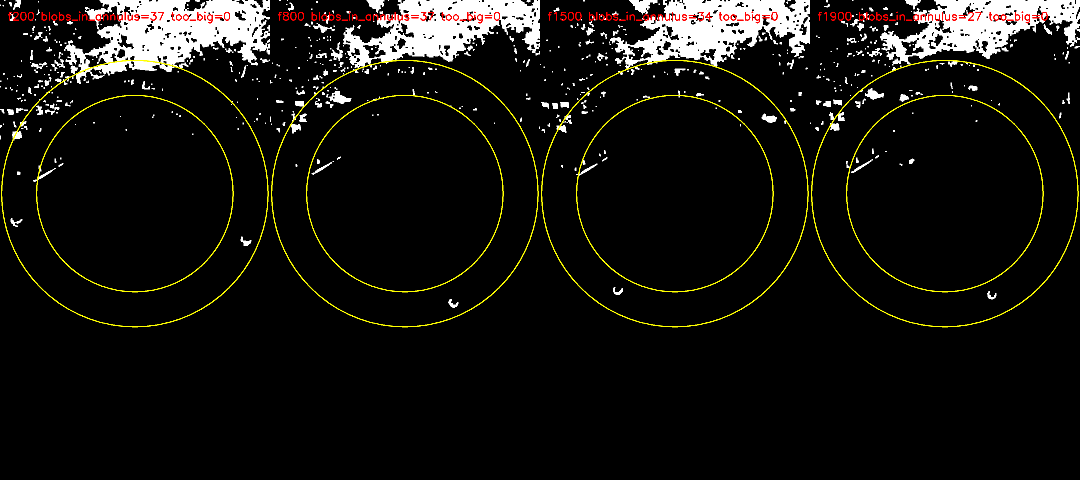
\includegraphics[width=\linewidth]{fig-mask-4048.png}
\caption{\texttt{roundabout-4048}: the HSV ``dark'' mask with the rim annulus overlaid. The
entire top of every frame is foliage passing the same threshold as the knob, and the orbit runs
straight through it.}
\label{fig:mask4048}
\end{figure}

%======================================================================
\textbf{Verdict: REJECTED (archived).} The information is absent from the pixels; the clip needs a
re-shoot, not a parameter.

\section{Cross-corpus findings}

\subsection{Perspective is \emph{not} systematic --- a retraction, and the rule that replaced it}
\label{sec:null}

An earlier draft of this report claimed that perspective was a corpus-level property, on the
grounds that three unrelated rigs (4046, bicycle, turntable-1) all showed a mixed $A_1/A_2$
fingerprint and a ripple CV in a narrow $0.159$--$0.168$ band. \textbf{That claim was wrong and
is retracted.} It was produced by a classifier that read the harmonic \emph{ratio} without
testing whether the ripple was phase-locked at all. A ratio computed on noise is still a ratio.

Running the rectification on the two additional clips falsified it directly
(Table~\ref{tab:null}).

\begin{table}[htbp]
\centering
\footnotesize
\begin{tabular}{lrrrrrl}
\toprule
Clip & Tilt & \textbf{Hub offset} & Revs & Phase-lock & ripple CV (before $\to$ after) & Outcome \\
\midrule
roundabout-4046   & $27.1^\circ$ & \textbf{85.6\,px} & 18.6 & \textbf{0.94} & $0.166 \to \mathbf{0.015}$ & fixed \\
bicycle           & $15.0^\circ$ & 4.9\,px  & 6.4 & 0.72 & $0.141 \to 0.148$ & no effect \\
turntable-1       & $14.9^\circ$ & 8.8\,px  & 2.6 & 0.15 & $0.159 \to 0.162$ & no artifact \\
turntable-2       & $11.3^\circ$ & 3.4\,px  & 1.4 & 0.58$^\dag$ & --- & no perspective \\
turntable-3/flick & $3.8^\circ$  & \textbf{0.7\,px} & 1.8 & 0.40$^\dag$ & --- & no perspective \\
\bottomrule
\end{tabular}
\caption{The null results. $^\dag$Below 2 revolutions the phase-lock statistic fits four
harmonics to $\sim$1.5 cycles and is not meaningful. Rectification helps exactly one clip, and
the hub offset predicts which one \emph{in advance}.}
\label{tab:null}
\end{table}

\textbf{The rule that replaced it: perspective strength is the hub offset, not the tilt.} The
offset between the imaged axle and the centre of the elliptical path is $85.6$\,px on 4046 and
$0.7$--$8.8$\,px on every other clip --- an order-of-magnitude separation, with 4046 alone on
one side. This is not a coincidence of thresholds: the offset \emph{is} the perspective
(\S\ref{sec:trap}), so a near-zero offset means the view is essentially affine, the vanishing
line lies near infinity, the recovered homography is near-identity, and there is nothing to
undo. The rectification did nothing on four clips because \emph{nothing was wrong with them}.

Tilt does not predict this. All five clips are tilted, three of them by $15$--$27^\circ$. Tilt
determines only that the orbit \emph{images} as an ellipse; whether that ellipse is an affine or
a projective image of the circle depends on the camera's distance relative to the orbit --- 4046
was shot close with a wide phone lens, the others flatter. \textbf{An affine ellipse needs no
un-projection: $\theta$ read from a correctly-centred ellipse is already right.}

\subsection{What the corpus does support}

\begin{itemize}
  \item \textbf{One clip} (\texttt{roundabout-4046}) carries a large, genuinely phase-locked
  ($0.94$ over 18.6 revolutions) perspective artifact, and it is removable.
  \item \textbf{The fans' $0.0^\circ$ entries are not evidence of good capture} --- their orbits
  are synthesized. The two clips that look cleanest in the corpus are the two that are not
  measurements.
  \item \textbf{An unexplained result:} \texttt{bicycle}'s ripple \emph{is} phase-locked
  ($0.72$ over 6.4 revolutions) but is not perspective (offset $4.9$\,px) and is not periodic
  occlusion (visible area versus orbital phase gives $R^2 = 0.073$). Rectification makes it
  marginally worse. The cause is unknown. It tracks an extended object (a whole phone threaded
  through the spokes), so a centroid effect is a hypothesis, not a finding.
\end{itemize}

\textbf{Phase-lock proves orbit-synchrony, not projection.} Any effect locked to orbital phase
--- occlusion, an extended object's centroid, periodic lighting --- produces the same signature.
The fingerprint of \S\ref{sec:fingerprint} narrows the candidates; only the hub offset, measured
independently of the kinematics, distinguishes perspective among them. A diagnostic that skips
that check will misattribute noise to geometry, which is exactly what happened here.

\subsection{Tracker provenance: the golden set spans both backends}
\label{sec:backends}

\begin{center}
\begin{tabular}{lll}
\toprule
Phenomenon & Tracker & Cache \texttt{method} \\
\midrule
roundabout-4046 & SAM3 (text-conditioned) & \texttt{sam3\_object} \\
turntable 1/2/3 & SAM3 & (no cache; fetched fresh) \\
computerfan-4029 & \textbf{colour} (local, CPU) & \texttt{color} \\
fan-4027/4028 & \emph{neither} & \texttt{frequency\_synth\_windowed} \\
roundabout-4048 & colour & \texttt{color} \\
\bottomrule
\end{tabular}
\end{center}

\textbf{The findings are not backend-specific.} 4046's perspective artifact arrived through SAM3
and 4029's clean data through the colour tracker, and both were judged by identical criteria ---
the hub offset, the harmonic fingerprint and the angular step bound all operate on the
\emph{trajectory}, not on the tracker. The fans' \texttt{frequency\_synth\_windowed} also
confirms from the cache itself, rather than by inference, that their orbits are synthesized.

\textbf{A provenance gap.} The remote \texttt{/track} API returns \texttt{status},
\texttt{request\_id}, \texttt{video\_id}, \texttt{video\_info} and \texttt{trajectories}, and
\textbf{no \texttt{method} field}; \texttt{method} and \texttt{track\_coverage} are stamped on downstream, unevenly. Three
cache shapes coexist, and \texttt{flick}'s carries no provenance at all --- which is precisely
how the \texttt{flick} $=$ \texttt{turntable-3} duplicate stayed invisible. \textbf{A cache
should record the tracker, the tracker version, and a hash of the source video at write time.}

\textbf{Aside: SAM3 was deterministic here.} A fresh SAM3 fetch of \texttt{turntable-3} returned
a track \textbf{byte-identical} to \texttt{flick}'s cache (350/350 points, both objects, exact
float equality) --- which is how \texttt{flick}'s provenance was established. The orchestrator's
hard rules assume SAM3 is non-deterministic and wrap it in a bounded-retry loop; that premise did
not hold on this clip. One clip is not a general claim, but the assumption deserves a test.

\subsection{Detection fails by prompt--shape collision}

Three of ten real tracks are unusable, and every failure has the same mechanism: \textbf{the
prompt noun names a shape or colour that the background also contains.}

\begin{center}
\begin{tabular}{lll}
\toprule
Clip & Prompt & Actually tracked \\
\midrule
fan-doll         & \texttt{"fan blade"}   & the window's louvre slats \\
roundabout-4048  & \texttt{"black knob"}  & dark foliage \\
computerfan-4029 & \texttt{"red marker"}  & unverified; 153 teleports \\
\bottomrule
\end{tabular}
\end{center}

Existing lab guidance holds that simple category nouns track better than elaborate
descriptions. This corpus adds a sharper, partly opposing rule: \textbf{a noun that describes a
shape will find that shape in the background.} \texttt{"fan blade"} is an excellent description
of a window louvre. The failure is not that the prompt is too complex --- it is that the prompt
is not \emph{discriminative within the frame}. A prompt must be chosen against the background,
not against the object alone.

\textbf{The same rule governs the colour backend, with ``feature'' redefined.} SAM3 fails by
semantic/shape collision; colour tracking fails by hue/value collision (\texttt{"black knob"}
against foliage; a cream toy against a cream ceiling). Both reduce to: \emph{the target's
defining feature is shared with the background}. \texttt{fan-doll} fails on \textbf{both}
backends because its toy is semantically hard \emph{and} cream-on-cream --- which is why
switching tracker did not save it, and only a physical marker will.

\subsection{Coverage is not correctness}

\texttt{roundabout-4048} reports \texttt{track\_coverage: 1.0} while being wrong in
$\sim$38\% of frames. Coverage measures whether the tracker returned a point, not whether the
point is the object. Every quality gate keyed on coverage will pass this clip. The gate that
catches it is box-area stability combined with a physically-derived step bound.

%======================================================================
\section{The golden set: what we can vouch for}
\label{sec:golden}

``Golden'' means \emph{we know this clip's data is right} --- not that it is pretty. Four
phenomena qualify, in two tiers:
\begin{itemize}
  \item \textbf{GOLD} --- the per-frame \emph{trajectory} is measured, so every quantity (position,
  $\omega$, $v$, $a_c$) is a direct observation.
  \item \textbf{SILVER} --- the \emph{rate} and \emph{scale} are measured, so $\omega$, $T$, $f$,
  $v$ and $a_c$ are trustworthy and teachable, but the per-frame \emph{trajectory} is reconstructed
  from the rate and must never be presented as measured data. (``Gold numbers, reconstructed
  picture.'')
\end{itemize}
The reason each clip fails or passes is specific.

\begin{center}
\begin{tabular}{llp{7.4cm}}
\toprule
Phenomenon & Status & Basis \\
\midrule
\textbf{roundabout-4046} & \textbf{GOLD} (corrected) & Track verified. Strong perspective
(hub offset 85.6\,px, phase-lock 0.94 over 18.6 rev) removed by rectification; mean $\omega$
invariant; circularity improved unoptimised. \\
\textbf{turntable} (1/2/3) & \textbf{GOLD} (as-is) & Tracks verified. Hub offsets
$0.7$--$8.8$\,px $\Rightarrow$ perspective geometrically impossible; t-1 phase-lock 0.15
$\Rightarrow$ ripple is broadband noise. \textbf{t-1 is a negative control}: tilted $14.9^\circ$
yet already correct, so a gate must provably \emph{not} fire on it. \\
\textbf{computerfan-4029} & \textbf{GOLD} (as-is) & Track verified; the SUSPECT verdict was our
gate's false positive (\S\ref{sec:4029}). Hub 99.4\%, offset 8.5\,px, ripple CV 0.088,
phase-lock 0.075. \\
\textbf{ceiling fan} (4027+4028) & \textbf{SILVER} & Rate verified against the real red marker
(corr 0.974); \emph{scale measured} (ruler: tip $63.5$\,cm $\Rightarrow$ $559$\,px/m), so $v$/$a_c$
at the blade tip are now real ($a_c$ peak $11.3$/$85.2$\,m/s$^2$); $\omega(t)$ staircase removed by
sub-bin interpolation. But the per-frame orbit is \emph{synthesized} from the rate --- teach the
numbers, never present the orbit as measured (\S\ref{sec:fans}). \\
\midrule
bicycle & \textcolor{warn}{open} & Track clean, but a phase-locked ($0.72$) ripple that is not
perspective ($4.9$\,px), not occlusion ($R^2 = 0.07$), and not cleanly gravity (right sign,
phase $138^\circ$ off). Cause unknown $\Rightarrow$ we cannot say what its data should be. Its
scale is also \emph{estimated} (no \texttt{physical\_size} in the sidecar) and a phone-vs-tire
cross-check disagrees by 12\% (\S\ref{sec:scale}). \\
fan-doll & \textcolor{bad}{no} & Cream toy on a cream ceiling. Green-sprout colour tracking
reaches only 51.7\% (\S\ref{sec:fandoll}). \\
roundabout-4048 & \textcolor{bad}{no} & Information absent from the pixels; archived for
re-shoot. \\
\bottomrule
\end{tabular}
\end{center}

\textbf{Four phenomena, and only one needed correcting.} That asymmetry is the report's
practical result: the corpus is mostly \emph{already right}, one clip was badly wrong in a way a
filter was hiding, and two are wrong in ways no processing reaches. Distinguishing those states
--- not any single fix --- is what the pipeline needs to be able to do.

\textbf{Three of the four were obtained by correcting our own diagnostics or configuration, not
by touching the data.} 4029 was cleared by replacing a pixel step threshold with an angular one
(\S\ref{sec:4029}); the turntables by the hub offset, a static measurement needing no revolutions;
and the fans by measuring the blade-tip scale with a ruler and smoothing the FFT-quantised rate ---
the blade-pass $\omega$ having been right all along (\S\ref{sec:fans}). Only
\texttt{roundabout-4046} required an actual correction to the data. \textbf{The dominant failure mode in this investigation was our own measurement, not the
capture.}

%======================================================================
\section{The rectification method}
\label{sec:method-rect}

\subsection{Why the obvious fix fails}
\label{sec:affine}

The natural reading --- ``filmed at an angle, so the circle images as an ellipse; stretch it
back'' --- is a \emph{weak-perspective} (affine) model. It predicts a pure 2/rev ripple, because
foreshortening is symmetric: the orbit crosses the major axis twice per revolution.

\texttt{roundabout-4046} shows a dominant \textbf{1}/rev term (Figure~\ref{fig:fingerprint}),
which affine tilt cannot produce at all. Its origin is true perspective: the near side of the
orbit is magnified relative to the far side, an asymmetry with a once-per-revolution period.
Applying the affine fix there moved the ripple CV from $0.166$ to only $0.146$ --- a 12\%
improvement (Figure~\ref{fig:affinefail}), because it addresses the smaller of the two harmonics
and leaves the larger untouched.

This reasoning applies \emph{only} where perspective is actually present. On the four clips whose
hub offset is near zero (\S\ref{sec:null}) the image \emph{is} an affine view of the circle, the
axis stretch is the correct and sufficient model, and no projective step is warranted.

\begin{figure}[htbp]
\centering
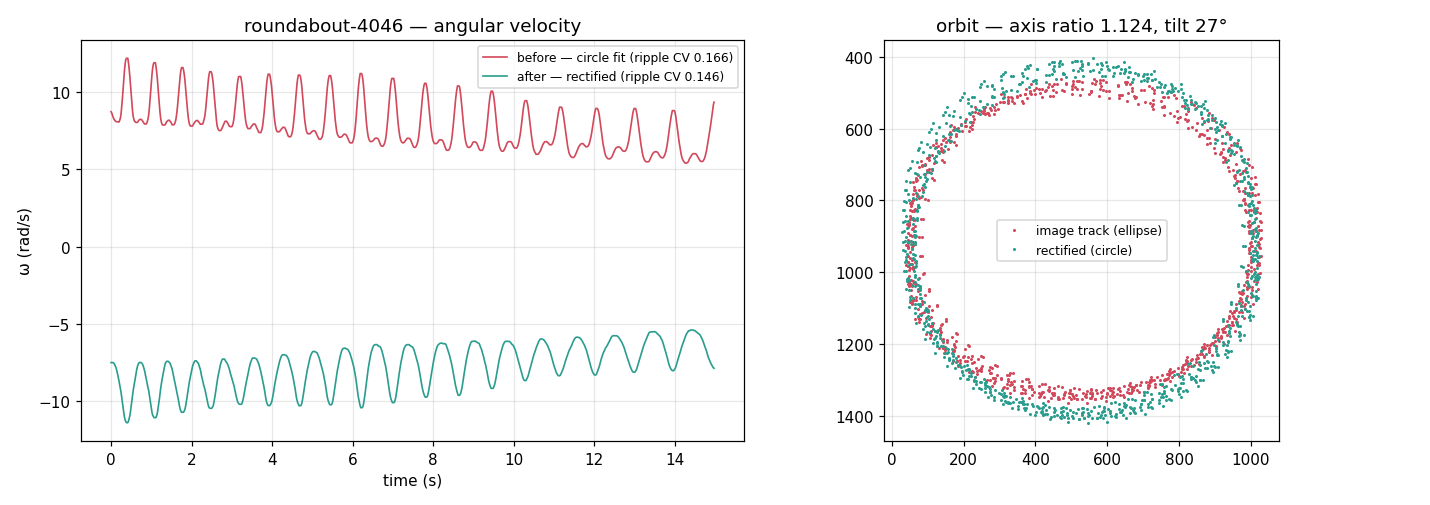
\includegraphics[width=\linewidth]{fig-affine-fail-4046.png}
\caption{The affine remedy failing on \texttt{roundabout-4046}. The ripple survives at nearly
full amplitude (the sign flip is a handedness artifact of the eigenbasis, later corrected). The
peaks are spaced one revolution apart --- the signature affine rectification cannot address.}
\label{fig:affinefail}
\end{figure}

\subsection{Uncalibrated projective rectification via the vanishing line}

The enabling geometry: \textbf{for a circle, the polar line of the circle's centre with respect
to the circle is that plane's line at infinity.} Both the conic and the centre survive
projection, so the imaged rotation axle together with the fitted orbit conic yield the vanishing
line directly --- with \textbf{no camera intrinsics, no focal length, no EXIF}:

\begin{lstlisting}[language=Python]
C = fit_conic(orbit_x, orbit_y)      # image of the orbit (an ellipse)
h = (hub_x, hub_y, 1)                # the IMAGED AXLE -- not the ellipse centre
l = C @ h                            # polar of h = the plane's vanishing line
H = [[1,0,0], [0,1,0], [l0,l1,l2]]   # maps l to infinity -> now an AFFINE image
                                     # then ellipse -> circle by the axis stretch
theta = atan2(...)                   # in the metric-rectified plane
\end{lstlisting}

\subsection{The trap: the hub is not the centre of the ellipse}
\label{sec:trap}

This is the single way to get the method wrong, and it fails silently. On 4046:

\begin{center}
\begin{tabular}{lr}
\toprule
Centre of the elliptical path & $(530.0,\ 912.3)$ \\
The actual red axle boss (detected) & $(532.3,\ 997.9)$ --- \textbf{85.6\,px lower} \\
\texttt{sidecar.rotation\_center\_frac} & $(529.5,\ 909.7)$ --- \emph{2.6\,px from the ellipse centre} \\
\bottomrule
\end{tabular}
\end{center}

These two points coincide \emph{only} under affine viewing. Their offset \textbf{is} the
perspective, and it is the method's entire input. Pass the ellipse centre as $h$ and the polar
returns the line at infinity, the homography is the identity, and the rectification silently
does nothing.

This has a direct consequence for the sidecar: \textbf{\texttt{rotation\_center\_frac} is
unusable as $h$}. A human asked to ``mark the centre'' taps the middle of the ring they see ---
which is exactly the point carrying no information. The axle must be detected instead. On 4046
this is reliable: the dark-red boss (HSV $\approx$ (0--10 / 170--179, 120--255, 40--160),
roundish, nearest the orbit centre) was found in \textbf{100\% of frames}
(Figure~\ref{fig:hub}). Tracking it per frame also absorbs camera drift for free.

\begin{figure}[htbp]
\centering
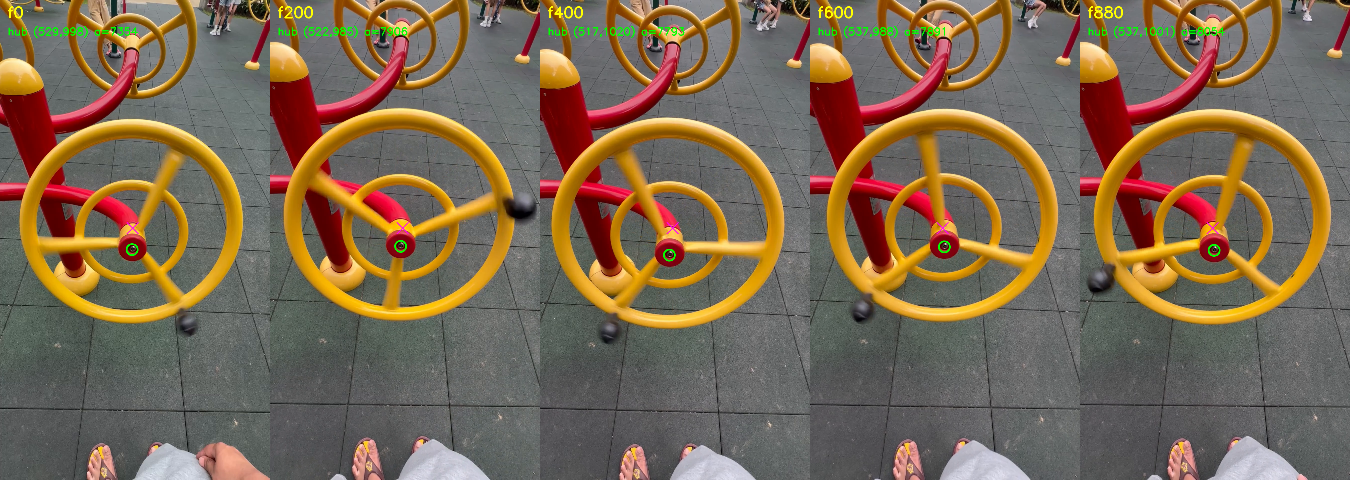
\includegraphics[width=\linewidth]{fig-hub-4046.png}
\caption{Axle detection on \texttt{roundabout-4046}, 100\% of frames. Green circle: the detected
red hub. Magenta cross: the sidecar's marked ``centre'', which coincides with the centre of the
\emph{elliptical path}. The visible gap between them is the 85.6\,px perspective offset that
drives the rectification.}
\label{fig:hub}
\end{figure}

\subsection{Why this is not circular reasoning}

A sufficiently flexible transform can make any curve look nicer, so ``it got smoother'' is not
evidence. Two independent checks are required and both are reported:

\begin{itemize}
  \item \textbf{Mean $\omega$ must be preserved.} Rectification redistributes angle
  \emph{within} a revolution; it cannot change how many revolutions occurred, since a full
  revolution's average is projection-invariant. Measured: $7.799 \rightarrow 7.800$\,rad/s. A
  moving mean would indicate real signal being fitted away.
  \item \textbf{Circularity must improve without having been optimised.} The vanishing line is
  derived from the detected hub --- never from $\omega$, never from the radial residual. The
  residual falling $5.20\% \rightarrow 1.68\%$ is therefore a free, independent confirmation.
\end{itemize}

A rectification derived from the kinematics it then ``improves'' is worthless; any report of
this method should state which inputs came from geometry and which from motion.

\subsection{Independent corroboration}

The pipeline already contains an unrelated mitigation (\S\ref{sec:filter}): a 1-revolution
moving average. A boxcar of exactly one period cancels all harmonics of the orbital frequency,
so its trend is approximately correct by construction --- and it independently recovers
$9.5 \rightarrow 6.5$\,rad/s, against rectification's $9.4 \rightarrow 6.5$. Two unrelated
methods agreeing on the physics is meaningful support that the rectification recovers signal
rather than manufacturing it.

%======================================================================
\section{What the pipeline does today}
\label{sec:filter}

The current system \emph{already detects} this artifact and responds in two ways, both of which
treat the symptom:

\begin{enumerate}
  \item \textbf{A filter.} \texttt{render/figures.py} draws a 1-revolution moving average boldly
  over a faint raw trace. Its own comment reads: \emph{``Oblique-capture clip: the per-instant
  curve is a projection artifact. Show the raw values faintly and the 1-revolution trend boldly
  (the real physics).''}
  \item \textbf{A suppression rule.} \texttt{quality\_signals.py} computes the phase-lock
  fraction and, when the artifact is present, emits \texttt{do\_not\_claim} instructions
  forbidding the material generator from discussing per-instant $\omega$, the shape of the
  $\omega(t)$ curve, or any within-revolution variation.
\end{enumerate}

Both are reasonable given an uncorrected track, and the boxcar's trend is approximately right.
But the comparison is unfavourable on every axis that matters:

\begin{center}
\begin{tabular}{p{4.2cm}p{5.1cm}p{5.1cm}}
\toprule
 & 1-rev boxcar (current) & Projective rectification \\
\midrule
within-revolution $\omega$ & destroyed; may never be discussed & recovered (ripple CV 0.015) \\
cancellation & imperfect --- fixed window while the wheel decelerates & artifact removed at source \\
what the student sees & a bold line over a faint jagged trace, implying the raggedness is real & one clean line \\
material generation & \texttt{do\_not\_claim} suppression remains & suppression unnecessary \\
\bottomrule
\end{tabular}
\end{center}

The system is currently hiding an artifact it has enough information to remove.

%======================================================================
\section{Where each fix belongs}

An end-to-end test settled this. Per-clip guidance (\texttt{hints.md}) was injected verbatim
into the orchestrator prompt and the agent \emph{correctly ignored} the instruction to rectify,
because the orchestrator's hard rules state: \emph{``Kinematics is FROZEN. Never reimplement,
edit, or `improve' anything under \texttt{analysis/}.''} The freeze exists for good reason --- its
own docstrings record that agent-authored kinematics made \texttt{center\_drift} swing
8.9--1013\,px and \texttt{stable\_mean\_omega} swing 2.9--6.1\,rad/s \emph{on the same video}.

\textbf{This was not a model limitation. It was a misplaced hint.} The knowledge was filed in a
layer with no authority to act on it.

\begin{center}
\begin{tabular}{l p{6.6cm} l}
\toprule
Layer & Owns & Reachable by a hint? \\
\midrule
Steps 1--5 (agentic) & tracking mode, params, prompts, \textbf{hub detection}, refusal & \textbf{yes} \\
\texttt{pipeline\_inputs.json} & the contract seam --- carries per-clip measurements & \textbf{yes} \\
Step 6 \texttt{analysis/} (frozen) & calibration, geometry, kinematics, stats & \textbf{no --- by design} \\
\bottomrule
\end{tabular}
\end{center}

The proposed split follows directly, and matches the intended small-agent/large-agent
architecture: \textbf{the large agent supplies the method} (once, validated, as code);
\textbf{the small agent supplies the per-clip observation} (detect the axle, emit
\texttt{hub\_px} through the contract); \textbf{the frozen pipeline does the arithmetic}
(rectify when \texttt{hub\_px} is present and materially offset from the ellipse centre).
Nothing asks a 35B model to re-derive projective geometry per job, and the gate leaves
near-face-on clips bit-identical.

\subsection{A delivery bug worth recording}
\label{sec:survey-bugs}

An earlier attempt instructed the agent to read \texttt{hints.md} itself. It transcribed the
loading code into a generated script, emitted
\texttt{[Step 1] hints.md found (5484 chars) --- AUTHORITATIVE}, and \textbf{never read a word
of it} (zero tool calls). A log line asserting compliance is not compliance: text read into a
file handle at runtime is not text in the model's context. Guidance must be \emph{injected}
into the prompt, not made \emph{available} to the agent --- the pattern
\texttt{material\_tiers.py} already uses for \texttt{material\_hints.md}.

The survey tool itself failed twice in the same family: it initially classified the idle-then-
flick clip as ``perspective'' (dividing the ripple by a near-zero mean $\omega$ over a mostly
stationary clip) and profiled the static reference base as though it orbited. Both are
statistics computed over the wrong window --- the same error as the 4048 tilt, one level up.

%======================================================================
\section{Limitations}

\begin{itemize}
  \item \textbf{One clip carries the finding.} Perspective is validated, and fixed, on
  \texttt{roundabout-4046} alone. Four other clips were tested and show no perspective. The
  corpus supports ``4046 has a strong perspective artifact and the hub offset identifies it'',
  \emph{not} ``Centri's data is distorted by perspective''.
  \item \textbf{The hub-offset rule rests on a 5-clip separation} ($85.6$\,px versus
  $0.7$--$8.8$\,px). The gap is an order of magnitude and the physics behind it is sound, but no
  threshold has been calibrated, and no clip sits in between --- we have not seen an
  intermediate case.
  \item \textbf{\texttt{bicycle} is unexplained.} A phase-locked ripple that is neither
  perspective nor occlusion. Until it is understood, we cannot claim to know what that clip's
  data should be.
  \item \textbf{No external ground truth.} Everything rests on internal consistency (invariant
  mean $\omega$; an unoptimised circularity gain) and agreement with the pipeline's independent
  1-revolution boxcar. No independently measured $\omega$ --- a rated fan speed, a metronome, a
  hand-counted revolution --- anchors the corpus. \textbf{This is the most valuable missing
  piece.}
  \item \textbf{The corpus is thin and partly duplicated.} Eleven templates reduce to $\sim$six
  phenomena; \texttt{flick} $=$ \texttt{turntable-3}; \texttt{turntable-1/2/3} are one phenomenon;
  \texttt{fan-4027/4028} are one physical fan; two of ten tracks are unusable. \textbf{Four
  phenomena have data we can vouch for} (\S\ref{sec:golden}) --- and only one needed the data
  corrected.
  \item \textbf{One scale question remains open} and must not be guessed: the phone's body length
  (to settle bicycle's 12\% cross-check). The fan scale is now measured (blade tip $63.5$\,cm
  $\Rightarrow$ $559$\,px/m, \S\ref{sec:fans}), so the fans' $v$/$a_c$ are real; $\omega$/$T$/$f$ are
  scale-free throughout and never depended on it.
  \item \textbf{Two clips are undiagnosable by fingerprint} at 1.4 and 1.8 revolutions, though
  the hub offset --- a static measurement needing no revolutions --- still clears them of
  perspective. Future captures should target $\ge 3$ revolutions of sustained motion.
  \item \textbf{The unused footage adds little breadth.} \texttt{New cases/} holds 11 unused
  clips, but 4039--4044 are six more takes of 4046's wheel, 4047 is 4048's rig, and 4025/4026/4030
  are further fans. The only new phenomenon, \texttt{4031} (an object swung on a string), is
  untrackable: the object is a motion-blur streak on a hand-held pivot, and a \texttt{"pink
  object"} prompt returns 100\% coverage while tracking the \emph{centroid of the smear}. Corpus
  breadth requires new filming, not more processing.
  \item \textbf{The prompt-collision rule is descriptive.} It is drawn from three failures and
  has not been confirmed by re-prompting; the one attempt (\texttt{fan-doll}) failed for an
  unrelated reason.
\end{itemize}

\section{Recommendations}

\begin{enumerate}
  \item \textbf{Capture beats correction.} Every artifact here was cheaper to prevent than to
  fix. Film closer to face-on; ensure $\ge 3$ revolutions; choose a marker that contrasts with
  the \emph{background}, not merely with the object.
  \item \textbf{Implement rectification in \texttt{geometry.py}}, \textbf{gated on the hub
  offset} rather than on tilt, with the agent detecting the axle in Step 5 and passing
  \texttt{hub\_px} through \texttt{pipeline\_inputs.json}. The gate is the point: four of five
  clips must be left untouched and bit-identical. Accept that 4046's golden numbers will move
  --- the previous ones were wrong.
  \item \textbf{Fix the two \texttt{color\_track.py} bugs} (saturation scoring for dark targets;
  physically-derived \texttt{max\_step}) independently of 4048's fate.
  \item \textbf{Replace coverage with correctness} in the quality gate: box-area stability plus an
  \textbf{angular} step bound derived from $\omega r/\mathrm{fps}$. A fixed pixel threshold both
  misses real failures and manufactures false ones --- it wrongly condemned \texttt{4029}, a clip
  that turned out to be the cleanest in the corpus.
  \item \textbf{Make the visual check mandatory} before any geometry statistic is computed. It
  falsified two confident claims in this investigation and two bugs in its own tooling.
\end{enumerate}

\vfill
\footnotesize
\textbf{Reproduction.} All paths relative to \texttt{agent-backend/}.

\begin{tabular}{@{}ll@{}}
Diagnostic and evidence & \texttt{docs/tracking-data-quality-2026-07-15.md} \\
Working rectification prototype & \texttt{docs/figures/rectify\_prototype.py} \\
Per-clip guidance & \texttt{templates/*/hints.md} \\
Archived clip and re-shoot notes & \texttt{templates-reshoot/} \\
\end{tabular}

\end{document}
